\section{OD performance requirements}
\label{sec:simulated_od_requirements}
\par
As previously stated, the primary purpose of the OD is to act as an active veto for neutrons.
Practically, this means that there are a number of performance requirements that the OD has to meet, all of which can be found in \cite{LZ_TechnicalDesignReview_ref}.
A subset, which are addressed in this thesis, are presented in \autoref{tab:veto_requirements}.
R-160001 is defined for a 1 MeV neutron as that is the most likely neutron energy expected in the TPC (more on this later).
R-160005 is set to a 5\% impact so as not to reduce the exposure (and therefore discovery potential) of LZ too much.
The OD will always veto more non-neutron events than neutron events as the expected neutron rate is so low.
This is acceptable as a single neutron event is more dangerous to a WIMP search than many electron recoil events.
\begin{table}[]
    \centering
    \begin{tabular}{p{0.3\textwidth}p{0.6\textwidth}} %{ c | c {\textwidth} } 
    \hline
    {Requirement Number} & {Description} \\ \hline
    R-160001             & Detection efficiency of 95\% for a 1 MeV neutron that scatters once in the xenon \\
    R-160005             & Must not veto more than 5\% of the WIMP search live-time
    \end{tabular}
    \caption{Selection of the OD veto performance requirements. Adapted from Table 12.2.6 from \cite{LZ_TechnicalDesignReview_ref}}
    \label{tab:veto_requirements}
\end{table} 

\par
The veto method adopted by LZ is to act as a `dumb' veto, as no attempt will be made to determine the cause of light seen in the OD.
This means that a single scatter event in the TPC will be vetoed if, in that event, there is a signal seen in the OD which:
\begin{enumerate}
    \item has energy above some threshold.
    \item is within some time window of the scatter in the TPC. 
\end{enumerate}
The veto window and threshold are determined by the background rate in the OD in order to reduce the impact on live-time.
This does, however, need to be balanced to maintain a suitable veto efficiency, as not all neutron captures in the OD will result in high energy signals.
These are both explored in the remainder of this chapter in simulations.

\subsection{OD Backgrounds}
\label{sec:simulated_od_backgrounds}
\par
A background in the OD is any event that is not what it was designed to detect and veto - so any event that is not a neutron or $\gamma$ that has scattered once in the TPC.
There have been numerous pre-construction studies to determine the expected background rate in the OD including \cite{LZ_TechnicalDesignReview_ref,LZ_projected_sensitivity_paper_ref,sallyshaw_thesis_ref,scotthaselschwardt_thesis_ref,lz_od_taup_2019_ref}, with the expected rate varying wildly, from between 56 Hz and 230 Hz for events above 200 keV.
In order to make sense of it, the key backgrounds are explained here, and an expected rate in the OD is determined based on the latest information about the detector.

\subsubsection{GdLS impurities}
\par
As part of the radioassay for LZ discussed previously, a dedicated campaign was undertaken to determine the rate of backgrounds in the GdLS \cite{scotthaselschwardt_thesis_ref}.
This LS screener campaign was motivated by the need to measure the $^{14}$C rate, a low energy $\beta$-decay (156.5 keV), which would essentially set what the minimum veto energy threshold could be.
If the rate of $^{14}$C is too high and the veto energy threshold set too low, then a large portion of TPC events would be vetoed mistakenly.
In the LZ Technical Design Review (TDR), the proposed veto energy threshold was 100 keV \cite{LZ_TechnicalDesignReview_ref}.
The radioassay also considered various decay chains and rare metals; both measured via $\alpha$ decays.
\par
One of the key discoveries of the screener campaign was the high ${}^{235}$U rate, with the measured level far higher than the relative abundance of ${}^{235}$U to ${}^{238}$U would suggest (0.720\% and 99.274\% respectively), though is a feature seen in other experiments \cite{javierperez_thesis_ref,superkamiokande_neutron_tagging_ref}.
This prompted the decay chains to be probed as sub-chains of the full chain.
The full decay chains considered ($^{232}$Th, $^{235}$U and $^{238}$U) are shown in \autoref{fig:decay_chains} along with how the sub-chains were defined.
The results from the LS screener campaign are shown in \autoref{tab:gdls_assay_rates}.
\par
In comparing the non-doped LS to doped LS, it was deduced that many of the contaminants were introduced as part of the purification of the gadolinium that occurs as it is added to the LS \cite{scotthaselschwardt_thesis_ref}.
As such, the method of doping the LS was altered, which aimed to reduce the contamination.
This `improved purification' GdLS is what was used to fill the LZ OD.
Included in \autoref{tab:gdls_assay_rates} are estimates from \cite{scotthaselschwardt_thesis_ref} of how this change in purification method will affect the GdLS, but it is important to stress that it did not undergo a radioassay, so the true rate is not known.
\par
The highest individual decay rate is from ${}^{14}$C.
This prompted a change in the veto energy threshold to be above the ${}^{14}$C end-point and so set to 200 keV.
This value is then what has been used in sensitivity studies of LZ \cite{LZ_projected_sensitivity_paper_ref}.

\begin{table}[]
    \centering
    \begin{tabular}{c|c|c}
        \multirow{2}{*}{Isotope or Subchain}  &  \multicolumn{2}{c}{GdLS rates (mBq/kg)}      \\ 
                             &  LS Screener          & Improved Purification \\ \hline
        ${}^{238}$U$_{e}$      &  $< 1.04$             & $< 0.017$             \\ 
        ${}^{238}$U$_{m}$      &  $0.092\pm0.02$       & $0.010\pm0.004$       \\
        ${}^{235}$U$_{e}$      &  $0.011$              & $< 0.018$             \\
        ${}^{235}$U$_{l}$      &  $0.10\pm0.04$        & $< 0.012$             \\
        ${}^{232}$Th$_{e}$     &  $< 0.027$            & $< 0.0036$            \\
        ${}^{232}$Th$_{l}$     &  $< 0.020$            & $< 0.0030$            \\
        ${}^{40}$K           &  $< 0.22$             & $< 0.0092$            \\
        ${}^{138}$La         &  $< 0.0055$           & $< 0.0017$            \\
        ${}^{176}$Lu         &  $0.30\pm0.07$        & $0.0081\pm0.0018$     \\
        ${}^{152}$Gd       &  $1.61\pm0.08$        & $1.61\pm0.08$         \\
        ${}^{147}$Sm       &  $1.02\pm0.05$        & $1.02\pm0.05$         \\
        ${}^{14}$C         &  $4.77\pm0.098$       & $4.77\pm0.098$ 
    \end{tabular}
    \caption{Activities of GdLS components during LS Screener testing and those projected from an improved purification technique. Values from Table 4.9 and 6.11 of \cite{scotthaselschwardt_thesis_ref}}
    \label{tab:gdls_assay_rates}
\end{table}
\par
Another source that was measured in the GdLS radioassay was ${}^{7}$Be, with an activity of $<$2.69 mBq/kg \cite{scotthaselschwardt_thesis_ref}.
This has been purposefully ignored in \autoref{tab:gdls_assay_rates} as ${}^{7}$Be has a half-life of 50-days \cite{be7_decay_ref}.
Therefore it will not be a significant contributor to the OD rate a year after the GdLS cocktail is created.

\newcommand{\nodewidth}{1cm}
\newcommand{\textnodewidth}{0.2cm}
\newcommand{\nodeminimumwidth}{32pt}
\newcommand{\nodespacing}{10pt}


\begin{landscape}
\begin{figure}
    \centering
\begin{tikzpicture}
  [node distance=0.05cm,text centered, thick]
  \tikzstyle{every node}=[font=\fontsize{5}{5}\selectfont]
 
    % For 3 chains, need 13 across
 \node[draw, rectangle, inner sep=0pt, text width=\nodewidth, minimum height=0.1cm, minimum width=\nodeminimumwidth, ] (neptunium_node_minus1) {};   
 \node[draw, rectangle, inner sep=0pt, text width=\nodewidth, minimum height=0.1cm, minimum width=\nodeminimumwidth, right=of neptunium_node_minus1] (neptunium_node_0) {};
 \node[draw, rectangle, inner sep=0pt, text width=\nodewidth, minimum height=0.1cm, minimum width=\nodeminimumwidth, right=of neptunium_node_0] (neptunium_node_1) {};
 \node[draw, rectangle, inner sep=0pt, text width=\nodewidth, minimum height=0.1cm, minimum width=\nodeminimumwidth, right=of neptunium_node_1] (neptunium_node_2) {};
 \node[draw, rectangle, inner sep=0pt, text width=\nodewidth, minimum height=0.1cm, minimum width=\nodeminimumwidth, right=of neptunium_node_2] (neptunium_node_3) {};
 \node[draw, rectangle, inner sep=0pt, text width=\nodewidth, minimum height=0.1cm, minimum width=\nodeminimumwidth, right=of neptunium_node_3] (neptunium_node_4) {};
 \node[draw, rectangle, inner sep=0pt, text width=\nodewidth, minimum height=0.1cm, minimum width=\nodeminimumwidth, right=of neptunium_node_4] (neptunium_chain_sep_1) {};
 \node[draw, rectangle, inner sep=0pt, text width=\nodewidth, minimum height=0.1cm, minimum width=\nodeminimumwidth, right=of neptunium_chain_sep_1] (neptunium_node_5) {};
 \node[draw, rectangle, inner sep=0pt, text width=\nodewidth, minimum height=0.1cm, minimum width=\nodeminimumwidth, right=of neptunium_node_5] (neptunium_node_6) {};
 \node[draw, rectangle, inner sep=0pt, text width=\nodewidth, minimum height=0.1cm, minimum width=\nodeminimumwidth, right=of neptunium_node_6] (neptunium_node_7) {};
 \node[draw, rectangle, inner sep=0pt, text width=\nodewidth, minimum height=0.1cm, minimum width=\nodeminimumwidth, right=of neptunium_node_7] (neptunium_node_8) {};
 \node[draw, rectangle, inner sep=0pt, text width=\nodewidth, minimum height=0.1cm, minimum width=\nodeminimumwidth, right=of neptunium_node_8] (neptunium_node_9) {};
 \node[draw, rectangle, inner sep=0pt, text width=\nodewidth, minimum height=0.1cm, minimum width=\nodeminimumwidth, right=of neptunium_node_9] (neptunium_chain_sep_2) {};
 \node[draw, rectangle, inner sep=0pt, text width=\nodewidth, minimum height=0.1cm, minimum width=\nodeminimumwidth, right=of neptunium_chain_sep_2] (neptunium_node_10) {};
 \node[draw, rectangle, inner sep=0pt, text width=\nodewidth, minimum height=0.1cm, minimum width=\nodeminimumwidth, right=of neptunium_node_10] (neptunium_node_11) {};
 \node[draw, rectangle, inner sep=0pt, text width=\nodewidth, minimum height=0.1cm, minimum width=\nodeminimumwidth, right=of neptunium_node_11] (neptunium_node_12) {};
 \node[draw, rectangle, inner sep=0pt, text width=\nodewidth, minimum height=0.1cm, minimum width=\nodeminimumwidth, right=of neptunium_node_12] (neptunium_label_sep) {};
 \node[draw, rectangle, inner sep=0pt, text width=\nodewidth, minimum height=0.1cm, minimum width=\nodeminimumwidth, right=of neptunium_label_sep] (neptunium_sep_3) {};
    
 \node[circle, inner sep=0pt, text width=\nodewidth, minimum width=\nodeminimumwidth, below=of neptunium_node_minus1] (uranium_node_minus1) {};   
 \node[draw, circle, inner sep=0pt, text width=\nodewidth, minimum width=\nodeminimumwidth, below=of neptunium_node_0] (uranium_node_0) {${}^{234}_{92}$U $245e^{3}$y};
 \node[circle, inner sep=0pt, text width=\nodewidth, minimum width=\nodeminimumwidth, below=of neptunium_node_1] (uranium_node_1) {};
 \node[draw, circle, inner sep=0pt, text width=\nodewidth, minimum width=\nodeminimumwidth, below=of neptunium_node_2] (uranium_node_2) {${}^{238}_{92}$U $4.5e^{9}$y};
 \node[circle, inner sep=0pt, text width=\nodewidth, minimum width=\nodeminimumwidth, below=of neptunium_node_3] (uranium_node_3) {};
 \node[circle, inner sep=0pt, text width=\nodewidth, minimum width=\nodeminimumwidth, below=of neptunium_node_4] (uranium_node_4) {};
 \node[circle, inner sep=0pt, text width=\nodewidth, minimum width=\nodeminimumwidth, below=of neptunium_chain_sep_1] (uranium_chain_sep_1) {};
 \node[draw, circle, inner sep=0pt, text width=\nodewidth, minimum width=\nodeminimumwidth, below=of neptunium_node_5] (uranium_node_5) {${}^{235}_{92}$U $7.0e^{8}$y};
 \node[circle, inner sep=0pt, text width=\nodewidth, minimum width=\nodeminimumwidth, below=of neptunium_node_6] (uranium_node_6) {};
 \node[circle, inner sep=0pt, text width=\nodewidth, minimum width=\nodeminimumwidth, below=of neptunium_node_7] (uranium_node_7) {};
 \node[circle, inner sep=0pt, text width=\nodewidth, minimum width=\nodeminimumwidth, below=of neptunium_node_8] (uranium_node_8) {};
 \node[circle, inner sep=0pt, text width=\nodewidth, minimum width=\nodeminimumwidth, below=of neptunium_node_9] (uranium_node_9) {};
 \node[circle, inner sep=0pt, text width=\nodewidth, minimum width=\nodeminimumwidth, below=of neptunium_chain_sep_2] (uranium_chain_sep_2) {};
 \node[circle, inner sep=0pt, text width=\nodewidth, minimum width=\nodeminimumwidth, below=of neptunium_node_10] (uranium_node_10) {};
 \node[circle, inner sep=0pt, text width=\nodewidth, minimum width=\nodeminimumwidth, below=of neptunium_node_11] (uranium_node_11) {};
 \node[circle, inner sep=0pt, text width=\nodewidth, minimum width=\nodeminimumwidth, below=of neptunium_node_12] (uranium_node_12) {};
 \node[circle, inner sep=0pt, text width=\nodewidth, minimum width=\nodeminimumwidth, below=of neptunium_label_sep] (uranium_label_sep) {};
 \node[circle, inner sep=0pt, text width=\nodewidth, minimum width=\nodeminimumwidth, below=of neptunium_sep_3] (uranium_sep_3) {Uranium};

 \node[circle, inner sep=0pt, text width=\nodewidth, minimum width=\nodeminimumwidth, below=of uranium_node_minus1] (protactinium_node_minus1) {};
 \node[circle, inner sep=0pt, text width=\nodewidth, minimum width=\nodeminimumwidth, below=of uranium_node_0] (protactinium_node_0) {};
 \node[draw, circle, inner sep=0pt, text width=\nodewidth, minimum width=\nodeminimumwidth, below=of uranium_node_1] (protactinium_node_1) {${}^{234}_{91}$Pa $1.2$m};
 \node[circle, inner sep=0pt, text width=\nodewidth, minimum width=\nodeminimumwidth, below=of uranium_node_2] (protactinium_node_2) {};
 \node[circle, inner sep=0pt, text width=\nodewidth, minimum width=\nodeminimumwidth, below=of uranium_node_3] (protactinium_node_3) {};
 \node[circle, inner sep=0pt, text width=\nodewidth, minimum width=\nodeminimumwidth, below=of uranium_node_4] (protactinium_node_4) {};
 \node[circle, inner sep=0pt, text width=\nodewidth, minimum width=\nodeminimumwidth, below=of uranium_node_5] (protactinium_node_5) {};
 \node[draw, circle, inner sep=0pt, text width=\nodewidth, minimum width=\nodeminimumwidth, below=of uranium_node_6] (protactinium_node_6) {${}^{231}_{91}$Pa $3.3e^{4}$y};
 \node[circle, inner sep=0pt, text width=\nodewidth, minimum width=\nodeminimumwidth, below=of uranium_node_7] (protactinium_node_7) {};
 \node[circle, inner sep=0pt, text width=\nodewidth, minimum width=\nodeminimumwidth, below=of uranium_node_8] (protactinium_node_8) {};
 \node[circle, inner sep=0pt, text width=\nodewidth, minimum width=\nodeminimumwidth, below=of uranium_node_9] (protactinium_node_9) {};
 \node[circle, inner sep=0pt, text width=\nodewidth, minimum width=\nodeminimumwidth, below=of uranium_node_10] (protactinium_node_10) {};
 \node[circle, inner sep=0pt, text width=\nodewidth, minimum width=\nodeminimumwidth, below=of uranium_node_11] (protactinium_node_11) {};
 \node[circle, inner sep=0pt, text width=\nodewidth, minimum width=\nodeminimumwidth, below=of uranium_node_12] (protactinium_node_12) {};
 \node[circle, inner sep=0pt, text width=\nodewidth, minimum width=\nodeminimumwidth, below=of uranium_label_sep] (protactinium_label_sep) {};
 \node[circle, inner sep=0pt, text width=\nodewidth, minimum width=\nodeminimumwidth, below=of uranium_sep_3] (protactinium_sep_3) {Protactinium};

 \node[circle, inner sep=0pt, text width=\nodewidth, minimum width=\nodeminimumwidth, below=of protactinium_node_minus1] (thorium_node_minus1) {};
 \node[draw, circle, inner sep=0pt, text width=\nodewidth, minimum width=\nodeminimumwidth, below=of protactinium_node_0] (thorium_node_0) {${}^{230}_{90}$Th $75e^{3}$y};
 \node[circle, inner sep=0pt, text width=\nodewidth, minimum width=\nodeminimumwidth, below=of protactinium_node_1] (thorium_node_1) {};
 \node[draw, circle, inner sep=0pt, text width=\nodewidth, minimum width=\nodeminimumwidth, below=of protactinium_node_2] (thorium_node_2) {${}^{234}_{90}$Th $24.1$d};
 \node[circle, inner sep=0pt, text width=\nodewidth, minimum width=\nodeminimumwidth, below=of protactinium_node_3] (thorium_node_3) {};
 \node[circle, inner sep=0pt, text width=\nodewidth, minimum width=\nodeminimumwidth, below=of protactinium_node_4] (thorium_node_4) {};
 \node[draw, circle, inner sep=0pt, text width=\nodewidth, minimum width=\nodeminimumwidth, below=of protactinium_node_5] (thorium_node_5) {${}^{231}_{90}$Th $25.5$h};
 \node[circle, inner sep=0pt, text width=\nodewidth, minimum width=\nodeminimumwidth, below=of protactinium_node_6] (thorium_node_6) {};
 \node[draw, circle, inner sep=0pt, text width=\nodewidth, minimum width=\nodeminimumwidth, below=of protactinium_node_7] (thorium_node_7) {${}^{227}_{90}$Th $18.7$d};
 \node[circle, inner sep=0pt, text width=\nodewidth, minimum width=\nodeminimumwidth, below=of protactinium_node_8] (thorium_node_8) {};
 \node[circle, inner sep=0pt, text width=\nodewidth, minimum width=\nodeminimumwidth, below=of protactinium_node_9] (thorium_node_9) {};
 \node[draw, circle, inner sep=0pt, text width=\nodewidth, minimum width=\nodeminimumwidth, below=of protactinium_node_10] (thorium_node_10) {${}^{228}_{90}$Th $1.9$y};
 \node[circle, inner sep=0pt, text width=\nodewidth, minimum width=\nodeminimumwidth, below=of protactinium_node_11] (thorium_node_11) {};
 \node[draw, circle, inner sep=0pt, text width=\nodewidth, minimum width=\nodeminimumwidth, below=of protactinium_node_12] (thorium_node_12) {${}^{232}_{90}$Th $1.4e^{10}$y};
 \node[circle, inner sep=0pt, text width=\nodewidth, minimum width=\nodeminimumwidth, below=of protactinium_label_sep] (thorium_label_sep) {};
 \node[circle, inner sep=0pt, text width=\nodewidth, minimum width=\nodeminimumwidth, below=of protactinium_sep_3] (thorium_sep_3) {Thorium};

 \node[circle, inner sep=0pt, text width=\nodewidth, minimum width=\nodeminimumwidth, below=of thorium_node_minus1] (actinium_node_minus1) {};
 \node[circle, inner sep=0pt, text width=\nodewidth, minimum width=\nodeminimumwidth, below=of thorium_node_0] (actinium_node_0) {};
 \node[circle, inner sep=0pt, text width=\nodewidth, minimum width=\nodeminimumwidth, below=of thorium_node_1] (actinium_node_1) {};
 \node[circle, inner sep=0pt, text width=\nodewidth, minimum width=\nodeminimumwidth, below=of thorium_node_2] (actinium_node_2) {};
 \node[circle, inner sep=0pt, text width=\nodewidth, minimum width=\nodeminimumwidth, below=of thorium_node_3] (actinium_node_3) {};
 \node[circle, inner sep=0pt, text width=\nodewidth, minimum width=\nodeminimumwidth, below=of thorium_node_4] (actinium_node_4) {};
 \node[circle, inner sep=0pt, text width=\nodewidth, minimum width=\nodeminimumwidth, below=of thorium_node_5] (actinium_node_5) {};
 \node[draw, circle, inner sep=0pt, text width=\nodewidth, minimum width=\nodeminimumwidth, below=of thorium_node_6] (actinium_node_6) {${}^{227}_{89}$Ac $21.8$y};
 \node[circle, inner sep=0pt, text width=\nodewidth, minimum width=\nodeminimumwidth, below=of thorium_node_7] (actinium_node_7) {};
 \node[circle, inner sep=0pt, text width=\nodewidth, minimum width=\nodeminimumwidth, below=of thorium_node_8] (actinium_node_8) {};
 \node[circle, inner sep=0pt, text width=\nodewidth, minimum width=\nodeminimumwidth, below=of thorium_node_9] (actinium_node_9) {};
 \node[circle, inner sep=0pt, text width=\nodewidth, minimum width=\nodeminimumwidth, below=of thorium_node_10] (actinium_node_10) {};
 \node[draw, circle, inner sep=0pt, text width=\nodewidth, minimum width=\nodeminimumwidth, below=of thorium_node_11] (actinium_node_11) {${}^{228}_{89}$Ac $6.1$h};
 \node[circle, inner sep=0pt, text width=\nodewidth, minimum width=\nodeminimumwidth, below=of thorium_node_12] (actinium_node_12) {};
 \node[circle, inner sep=0pt, text width=\nodewidth, minimum width=\nodeminimumwidth, below=of thorium_label_sep] (actinium_label_sep) {};
 \node[circle, inner sep=0pt, text width=\nodewidth, minimum width=\nodeminimumwidth, below=of thorium_sep_3] (actinium_sep_3) {Actinium}; 

 \node[circle, inner sep=0pt, text width=\nodewidth, minimum width=\nodeminimumwidth, below=of actinium_node_minus1] (radium_node_minus1) {};
 \node[draw, circle, inner sep=0pt, text width=\nodewidth, minimum width=\nodeminimumwidth, below=of actinium_node_0] (radium_node_0) {${}^{226}_{89}$Ra $1.6e^{3}$y};
 \node[circle, inner sep=0pt, text width=\nodewidth, minimum width=\nodeminimumwidth, below=of actinium_node_1] (radium_node_1) {};
 \node[circle, inner sep=0pt, text width=\nodewidth, minimum width=\nodeminimumwidth, below=of actinium_node_2] (radium_node_2) {};
 \node[circle, inner sep=0pt, text width=\nodewidth, minimum width=\nodeminimumwidth, below=of actinium_node_3] (radium_node_3) {};
 \node[circle, inner sep=0pt, text width=\nodewidth, minimum width=\nodeminimumwidth, below=of actinium_node_4] (radium_node_4) {};
 \node[circle, inner sep=0pt, text width=\nodewidth, minimum width=\nodeminimumwidth, below=of actinium_node_5] (radium_node_5) {};
 \node[circle, inner sep=0pt, text width=\nodewidth, minimum width=\nodeminimumwidth, below=of actinium_node_6] (radium_node_6) {};
 \node[draw, circle, inner sep=0pt, text width=\nodewidth, minimum width=\nodeminimumwidth, below=of actinium_node_7] (radium_node_7) {${}^{223}_{88}$Ra $11.4$d};
 \node[circle, inner sep=0pt, text width=\nodewidth, minimum width=\nodeminimumwidth, below=of actinium_node_8] (radium_node_8) {};
 \node[circle, inner sep=0pt, text width=\nodewidth, minimum width=\nodeminimumwidth, below=of actinium_node_9] (radium_node_9) {};
 \node[draw, circle, inner sep=0pt, text width=\nodewidth, minimum width=\nodeminimumwidth, below=of actinium_node_10] (radium_node_10) {${}^{224}_{88}$Ra $3.6$d};
 \node[circle, inner sep=0pt, text width=\nodewidth, minimum width=\nodeminimumwidth, below=of actinium_node_11] (radium_node_11) {};
 \node[draw, circle, inner sep=0pt, text width=\nodewidth, minimum width=\nodeminimumwidth, below=of actinium_node_12] (radium_node_12) {${}^{228}_{88}$Ra $5.7$y};
 \node[circle, inner sep=0pt, text width=\nodewidth, minimum width=\nodeminimumwidth, below=of actinium_label_sep] (radium_label_sep) {};
 \node[circle, inner sep=0pt, text width=\nodewidth, minimum width=\nodeminimumwidth, below=of actinium_sep_3] (radium_sep_3) {Radium}; 

 \node[circle, inner sep=0pt, text width=\nodewidth, minimum width=\nodeminimumwidth, below=of radium_node_minus1] (francium_node_minus1) {};
 \node[circle, inner sep=0pt, text width=\nodewidth, minimum width=\nodeminimumwidth, below=of radium_node_0] (francium_node_0) {};
 \node[circle, inner sep=0pt, text width=\nodewidth, minimum width=\nodeminimumwidth, below=of radium_node_1] (francium_node_1) {};
 \node[circle, inner sep=0pt, text width=\nodewidth, minimum width=\nodeminimumwidth, below=of radium_node_2] (francium_node_2) {};
 \node[circle, inner sep=0pt, text width=\nodewidth, minimum width=\nodeminimumwidth, below=of radium_node_3] (francium_node_3) {};
 \node[circle, inner sep=0pt, text width=\nodewidth, minimum width=\nodeminimumwidth, below=of radium_node_4] (francium_node_4) {};
 \node[circle, inner sep=0pt, text width=\nodewidth, minimum width=\nodeminimumwidth, below=of radium_node_5] (francium_node_5) {};
 \node[draw, circle, inner sep=0pt, text width=\nodewidth, minimum width=\nodeminimumwidth, below=of radium_node_6] (francium_node_6) {${}^{223}_{87}$Fr $22.0$m};
 \node[circle, inner sep=0pt, text width=\nodewidth, minimum width=\nodeminimumwidth, below=of radium_node_7] (francium_node_7) {};
 \node[circle, inner sep=0pt, text width=\nodewidth, minimum width=\nodeminimumwidth, below=of radium_node_8] (francium_node_8) {};
 \node[circle, inner sep=0pt, text width=\nodewidth, minimum width=\nodeminimumwidth, below=of radium_node_9] (francium_node_9) {};
 \node[circle, inner sep=0pt, text width=\nodewidth, minimum width=\nodeminimumwidth, below=of radium_node_10] (francium_node_10) {};
 \node[circle, inner sep=0pt, text width=\nodewidth, minimum width=\nodeminimumwidth, below=of radium_node_11] (francium_node_11) {};
 \node[circle, inner sep=0pt, text width=\nodewidth, minimum width=\nodeminimumwidth, below=of radium_node_12] (francium_node_12) {};
 \node[circle, inner sep=0pt, text width=\nodewidth, minimum width=\nodeminimumwidth, below=of radium_label_sep] (francium_label_sep) {};
 \node[circle, inner sep=0pt, text width=\nodewidth, minimum width=\nodeminimumwidth, below=of radium_sep_3] (francium_sep_3) {Francium}; 

 \node[circle, inner sep=0pt, text width=\nodewidth, minimum width=\nodeminimumwidth, below=of francium_node_minus1] (radon_node_minus1) {};
 \node[draw, circle, inner sep=0pt, text width=\nodewidth, minimum width=\nodeminimumwidth, below=of francium_node_0] (radon_node_0) {${}^{222}_{86}$Rn $3.8$d};
 \node[circle, inner sep=0pt, text width=\nodewidth, minimum width=\nodeminimumwidth, below=of francium_node_1] (radon_node_1) {};
 \node[circle, inner sep=0pt, text width=\nodewidth, minimum width=\nodeminimumwidth, below=of francium_node_2] (radon_node_2) {};
 \node[circle, inner sep=0pt, text width=\nodewidth, minimum width=\nodeminimumwidth, below=of francium_node_3] (radon_node_3) {};
 \node[circle, inner sep=0pt, text width=\nodewidth, minimum width=\nodeminimumwidth, below=of francium_node_4] (radon_node_4) {};
 \node[circle, inner sep=0pt, text width=\nodewidth, minimum width=\nodeminimumwidth, below=of francium_node_5] (radon_node_5) {};
 \node[circle, inner sep=0pt, text width=\nodewidth, minimum width=\nodeminimumwidth, below=of francium_node_6] (radon_node_6) {};
 \node[draw, circle, inner sep=0pt, text width=\nodewidth, minimum width=\nodeminimumwidth, below=of francium_node_7] (radon_node_7) {${}^{219}_{86}$Rn $4.0$s};
 \node[circle, inner sep=0pt, text width=\nodewidth, minimum width=\nodeminimumwidth, below=of francium_node_8] (radon_node_8) {};
 \node[circle, inner sep=0pt, text width=\nodewidth, minimum width=\nodeminimumwidth, below=of francium_node_9] (radon_node_9) {};
 \node[draw, circle, inner sep=0pt, text width=\nodewidth, minimum width=\nodeminimumwidth, below=of francium_node_10] (radon_node_10) {${}^{220}_{86}$Rn $55$s};
 \node[circle, inner sep=0pt, text width=\nodewidth, minimum width=\nodeminimumwidth, below=of francium_node_11] (radon_node_11) {};
 \node[circle, inner sep=0pt, text width=\nodewidth, minimum width=\nodeminimumwidth, below=of francium_node_12] (radon_node_12) {};
 \node[circle, inner sep=0pt, text width=\nodewidth, minimum width=\nodeminimumwidth, below=of francium_label_sep] (radon_label_sep) {};
 \node[circle, inner sep=0pt, text width=\nodewidth, minimum width=\nodeminimumwidth, below=of francium_sep_3] (radon_sep_3) {Radon}; 

 \node[circle, inner sep=0pt, text width=\nodewidth, minimum width=\nodeminimumwidth, below=of radon_node_minus1] (astatine_node_minus1) {};
 \node[circle, inner sep=0pt, text width=\nodewidth, minimum width=\nodeminimumwidth, below=of radon_node_0] (astatine_node_0) {};
 \node[draw, circle, inner sep=0pt, text width=\nodewidth, minimum width=\nodeminimumwidth, below=of radon_node_1] (astatine_node_1) {${}^{218}_{85}$At $1.5$s};
 \node[circle, inner sep=0pt, text width=\nodewidth, minimum width=\nodeminimumwidth, below=of radon_node_2] (astatine_node_2) {};
 \node[circle, inner sep=0pt, text width=\nodewidth, minimum width=\nodeminimumwidth, below=of radon_node_3] (astatine_node_3) {};
 \node[circle, inner sep=0pt, text width=\nodewidth, minimum width=\nodeminimumwidth, below=of radon_node_4] (astatine_node_4) {};
 \node[circle, inner sep=0pt, text width=\nodewidth, minimum width=\nodeminimumwidth, below=of radon_node_5] (astatine_node_5) {};
 \node[draw, circle, inner sep=0pt, text width=\nodewidth, minimum width=\nodeminimumwidth, below=of radon_node_6] (astatine_node_6) {${}^{219}_{85}$At $56$s};
 \node[circle, inner sep=0pt, text width=\nodewidth, minimum width=\nodeminimumwidth, below=of radon_node_7] (astatine_node_7) {};
 \node[draw, circle, inner sep=0pt, text width=\nodewidth, minimum width=\nodeminimumwidth, below=of radon_node_8] (astatine_node_8) {${}^{215}_{85}$At $1e^{-4}$s};
 \node[circle, inner sep=0pt, text width=\nodewidth, minimum width=\nodeminimumwidth, below=of radon_node_9] (astatine_node_9) {};
 \node[circle, inner sep=0pt, text width=\nodewidth, minimum width=\nodeminimumwidth, below=of radon_node_10] (astatine_node_10) {};
 \node[circle, inner sep=0pt, text width=\nodewidth, minimum width=\nodeminimumwidth, below=of radon_node_11] (astatine_node_11) {};
 \node[circle, inner sep=0pt, text width=\nodewidth, minimum width=\nodeminimumwidth, below=of radon_node_12] (astatine_node_12) {};
 \node[circle, inner sep=0pt, text width=\nodewidth, minimum width=\nodeminimumwidth, below=of radon_label_sep] (astatine_label_sep) {};
 \node[circle, inner sep=0pt, text width=\nodewidth, minimum width=\nodeminimumwidth, below=of radon_sep_3] (astatine_sep_3) {Astatine}; 

 \node[circle, inner sep=0pt, text width=\nodewidth, minimum width=\nodeminimumwidth, below=of astatine_node_minus1] (polonium_node_minus1) {};
 \node[draw, circle, inner sep=0pt, text width=\nodewidth, minimum width=\nodeminimumwidth, below=of astatine_node_0] (polonium_node_0) {${}^{218}_{84}$Po $3$m};
 \node[circle, inner sep=0pt, text width=\nodewidth, minimum width=\nodeminimumwidth, below=of astatine_node_1] (polonium_node_1) {};
 \node[draw, circle, inner sep=0pt, text width=\nodewidth, minimum width=\nodeminimumwidth, below=of astatine_node_2] (polonium_node_2) {${}^{214}_{84}$Po $2e^{-8}$s};
 \node[circle, inner sep=0pt, text width=\nodewidth, minimum width=\nodeminimumwidth, below=of astatine_node_3] (polonium_node_3) {};
 \node[draw, circle, inner sep=0pt, text width=\nodewidth, minimum width=\nodeminimumwidth, below=of astatine_node_4] (polonium_node_4) {${}^{210}_{84}$Po $138$d};
 \node[circle, inner sep=0pt, text width=\nodewidth, minimum width=\nodeminimumwidth, below=of astatine_node_5] (polonium_node_5) {};
 \node[circle, inner sep=0pt, text width=\nodewidth, minimum width=\nodeminimumwidth, below=of astatine_node_6] (polonium_node_6) {};
 \node[draw, circle, inner sep=0pt, text width=\nodewidth, minimum width=\nodeminimumwidth, below=of astatine_node_7] (polonium_node_7) {${}^{215}_{84}$Po $1.8e^{-3}$s};
 \node[circle, inner sep=0pt, text width=\nodewidth, minimum width=\nodeminimumwidth, below=of astatine_node_8] (polonium_node_8) {};
 \node[draw, circle, inner sep=0pt, text width=\nodewidth, minimum width=\nodeminimumwidth, below=of astatine_node_9] (polonium_node_9) {${}^{211}_{84}$Po $5e^{-5}$s};
 \node[draw, circle, inner sep=0pt, text width=\nodewidth, minimum width=\nodeminimumwidth, below=of astatine_node_10] (polonium_node_10) {${}^{216}_{84}$Po $0.14$s};
 \node[circle, inner sep=0pt, text width=\nodewidth, minimum width=\nodeminimumwidth, below=of astatine_node_11] (polonium_node_11) {};
 \node[draw, circle, inner sep=0pt, text width=\nodewidth, minimum width=\nodeminimumwidth, below=of astatine_node_12] (polonium_node_12) {${}^{212}_{84}$Po $3e^{-7}$s};
 \node[circle, inner sep=0pt, text width=\nodewidth, minimum width=\nodeminimumwidth, below=of astatine_label_sep] (polonium_label_sep) {};
 \node[circle, inner sep=0pt, text width=\nodewidth, minimum width=\nodeminimumwidth, below=of astatine_sep_3] (polonium_sep_3) {Polonium}; 

 \node[circle, inner sep=0pt, text width=\nodewidth, minimum width=\nodeminimumwidth, below=of polonium_node_minus1] (bismuth_node_minus1) {};
 \node[circle, inner sep=0pt, text width=\nodewidth, minimum width=\nodeminimumwidth, below=of polonium_node_0] (bismuth_node_0) {};
 \node[draw, circle, inner sep=0pt, text width=\nodewidth, minimum width=\nodeminimumwidth, below=of polonium_node_1] (bismuth_node_1) {${}^{214}_{83}$Bi $20$m};
 \node[circle, inner sep=0pt, text width=\nodewidth, minimum width=\nodeminimumwidth, below=of polonium_node_2] (bismuth_node_2) {};
 \node[draw, circle, inner sep=0pt, text width=\nodewidth, minimum width=\nodeminimumwidth, below=of polonium_node_3] (bismuth_node_3) {${}^{210}_{83}$Bi $138$d};
 \node[circle, inner sep=0pt, text width=\nodewidth, minimum width=\nodeminimumwidth, below=of polonium_node_4] (bismuth_node_4) {};
 \node[circle, inner sep=0pt, text width=\nodewidth, minimum width=\nodeminimumwidth, below=of polonium_node_5] (bismuth_node_5) {};
 \node[draw, circle, inner sep=0pt, text width=\nodewidth, minimum width=\nodeminimumwidth, below=of polonium_node_6] (bismuth_node_6) {${}^{215}_{83}$Bi $8$m};
 \node[circle, inner sep=0pt, text width=\nodewidth, minimum width=\nodeminimumwidth, below=of polonium_node_7] (bismuth_node_7) {};
 \node[draw, circle, inner sep=0pt, text width=\nodewidth, minimum width=\nodeminimumwidth, below=of polonium_node_8] (bismuth_node_8) {${}^{211}_{83}$Bi $2$m};
 \node[circle, inner sep=0pt, text width=\nodewidth, minimum width=\nodeminimumwidth, below=of polonium_node_9] (bismuth_node_9) {};
 \node[circle, inner sep=0pt, text width=\nodewidth, minimum width=\nodeminimumwidth, below=of polonium_node_10] (bismuth_node_10) {};
 \node[draw, circle, inner sep=0pt, text width=\nodewidth, minimum width=\nodeminimumwidth, below=of polonium_node_11] (bismuth_node_11) {${}^{212}_{83}$Bi $61$m};
 \node[circle, inner sep=0pt, text width=\nodewidth, minimum width=\nodeminimumwidth, below=of polonium_node_12] (bismuth_node_12) {};
 \node[circle, inner sep=0pt, text width=\nodewidth, minimum width=\nodeminimumwidth, below=of polonium_label_sep] (bismuth_label_sep) {};
 \node[circle, inner sep=0pt, text width=\nodewidth, minimum width=\nodeminimumwidth, below=of polonium_sep_3] (bismuth_sep_3) {Bismuth}; 

 \node[circle, inner sep=0pt, text width=\nodewidth, minimum width=\nodeminimumwidth, below=of bismuth_node_minus1] (lead_node_minus1) {};
 \node[draw, circle, inner sep=0pt, text width=\nodewidth, minimum width=\nodeminimumwidth, below=of bismuth_node_0] (lead_node_0) {${}^{214}_{82}$Pb $27$m};
 \node[circle, inner sep=0pt, text width=\nodewidth, minimum width=\nodeminimumwidth, below=of bismuth_node_1] (lead_node_1) {};
 \node[draw, circle, inner sep=0pt, text width=\nodewidth, minimum width=\nodeminimumwidth, below=of bismuth_node_2] (lead_node_2) {${}^{210}_{82}$Pb $22$y};
 \node[circle, inner sep=0pt, text width=\nodewidth, minimum width=\nodeminimumwidth, below=of bismuth_node_3] (lead_node_3) {};
 \node[draw, circle, inner sep=0pt, text width=\nodewidth, minimum width=\nodeminimumwidth, below=of bismuth_node_4] (lead_node_4) {${}^{206}_{82}$Pb stable};
 \node[circle, inner sep=0pt, text width=\nodewidth, minimum width=\nodeminimumwidth, below=of bismuth_node_5] (lead_node_5) {};
 \node[circle, inner sep=0pt, text width=\nodewidth, minimum width=\nodeminimumwidth, below=of bismuth_node_6] (lead_node_6) {};
 \node[draw, circle, inner sep=0pt, text width=\nodewidth, minimum width=\nodeminimumwidth, below=of bismuth_node_7] (lead_node_7) {${}^{211}_{82}$Pb $36$m};
 \node[circle, inner sep=0pt, text width=\nodewidth, minimum width=\nodeminimumwidth, below=of bismuth_node_8] (lead_node_8) {};
 \node[draw, circle, inner sep=0pt, text width=\nodewidth, minimum width=\nodeminimumwidth, below=of bismuth_node_9] (lead_node_9) {${}^{207}_{82}$Pb stable};
 \node[draw, circle, inner sep=0pt, text width=\nodewidth, minimum width=\nodeminimumwidth, below=of bismuth_node_10] (lead_node_10) {${}^{212}_{82}$Pb $11$h};
 \node[circle, inner sep=0pt, text width=\nodewidth, minimum width=\nodeminimumwidth, below=of bismuth_node_11] (lead_node_11) {};
 \node[draw, circle, inner sep=0pt, text width=\nodewidth, minimum width=\nodeminimumwidth, below=of bismuth_node_12] (lead_node_12) {${}^{208}_{82}$Pb stable};
 \node[circle, inner sep=0pt, text width=\nodewidth, minimum width=\nodeminimumwidth, below=of bismuth_label_sep] (lead_label_sep) {};
 \node[circle, inner sep=0pt, text width=\nodewidth, minimum width=\nodeminimumwidth, below=of bismuth_sep_3] (lead_sep_3) {Lead}; 

 \node[circle, inner sep=0pt, text width=\nodewidth, minimum width=\nodeminimumwidth, below=of lead_node_minus1] (thallium_node_minus1) {};
 \node[circle, inner sep=0pt, text width=\nodewidth, minimum width=\nodeminimumwidth, below=of lead_node_0] (thallium_node_0) {};
 \node[draw, circle, inner sep=0pt, text width=\nodewidth, minimum width=\nodeminimumwidth, below=of lead_node_1] (thallium_node_1) {${}^{210}_{81}$Tl $1$m};
 \node[circle, inner sep=0pt, text width=\nodewidth, minimum width=\nodeminimumwidth, below=of lead_node_2] (thallium_node_2) {};
 \node[draw, circle, inner sep=0pt, text width=\nodewidth, minimum width=\nodeminimumwidth, below=of lead_node_3] (thallium_node_3) {${}^{206}_{81}$Tl $4$m};
 \node[circle, inner sep=0pt, text width=\nodewidth, minimum width=\nodeminimumwidth, below=of lead_node_4] (thallium_node_4) {};
 \node[circle, inner sep=0pt, text width=\nodewidth, minimum width=\nodeminimumwidth, below=of lead_node_5] (thallium_node_5) {};
 \node[circle, inner sep=0pt, text width=\nodewidth, minimum width=\nodeminimumwidth, below=of lead_node_6] (thallium_node_6) {};
 \node[circle, inner sep=0pt, text width=\nodewidth, minimum width=\nodeminimumwidth, below=of lead_node_7] (thallium_node_7) {};
 \node[draw, circle, inner sep=0pt, text width=\nodewidth, minimum width=\nodeminimumwidth, below=of lead_node_8] (thallium_node_8) {${}^{207}_{81}$Tl $5$m};
 \node[circle, inner sep=0pt, text width=\nodewidth, minimum width=\nodeminimumwidth, below=of lead_node_9] (thallium_node_9) {};
 \node[circle, inner sep=0pt, text width=\nodewidth, minimum width=\nodeminimumwidth, below=of lead_node_10] (thallium_node_10) {};
 \node[draw, circle, inner sep=0pt, text width=\nodewidth, minimum width=\nodeminimumwidth, below=of lead_node_11] (thallium_node_11) {${}^{208}_{81}$Tl $3$m};
 \node[circle, inner sep=0pt, text width=\nodewidth, minimum width=\nodeminimumwidth, below=of lead_node_12] (thallium_node_12) {};
 \node[circle, inner sep=0pt, text width=\nodewidth, minimum width=\nodeminimumwidth, below=of lead_label_sep] (thallium_label_sep) {};
 \node[circle, inner sep=0pt, text width=\nodewidth, minimum width=\nodeminimumwidth, below=of lead_sep_3] (thallium_sep_3) {Thallium};

 \node[circle, inner sep=0pt, text width=\nodewidth, minimum width=\nodeminimumwidth, below=of thallium_node_minus1] (mercury_node_minus1) {};
 \node[circle, inner sep=0pt, text width=\nodewidth, minimum width=\nodeminimumwidth, below=of thallium_node_0] (mercury_node_0) {};
 \node[circle, inner sep=0pt, text width=\nodewidth, minimum width=\nodeminimumwidth, below=of thallium_node_1] (mercury_node_1) {};
 \node[draw, circle, inner sep=0pt, text width=\nodewidth, minimum width=\nodeminimumwidth, below=of thallium_node_2] (mercury_node_2) {${}^{206}_{80}$Hg $8$m};
 \node[circle, inner sep=0pt, text width=\nodewidth, minimum width=\nodeminimumwidth, below=of thallium_node_3] (mercury_node_3) {};
 \node[circle, inner sep=0pt, text width=\nodewidth, minimum width=\nodeminimumwidth, below=of thallium_node_4] (mercury_node_4) {};
 \node[circle, inner sep=0pt, text width=\nodewidth, minimum width=\nodeminimumwidth, below=of thallium_node_5] (mercury_node_5) {};
 \node[circle, inner sep=0pt, text width=\nodewidth, minimum width=\nodeminimumwidth, below=of thallium_node_6] (mercury_node_6) {};
 \node[circle, inner sep=0pt, text width=\nodewidth, minimum width=\nodeminimumwidth, below=of thallium_node_7] (mercury_node_7) {};
 \node[circle, inner sep=0pt, text width=\nodewidth, minimum width=\nodeminimumwidth, below=of thallium_node_8] (mercury_node_8) {};
 \node[circle, inner sep=0pt, text width=\nodewidth, minimum width=\nodeminimumwidth, below=of thallium_node_9] (mercury_node_9) {};
 \node[circle, inner sep=0pt, text width=\nodewidth, minimum width=\nodeminimumwidth, below=of thallium_node_10] (mercury_node_10) {};
 \node[circle, inner sep=0pt, text width=\nodewidth, minimum width=\nodeminimumwidth, below=of thallium_node_11] (mercury_node_11) {};
 \node[circle, inner sep=0pt, text width=\nodewidth, minimum width=\nodeminimumwidth, below=of thallium_node_12] (mercury_node_12) {};
 \node[circle, inner sep=0pt, text width=\nodewidth, minimum width=\nodeminimumwidth, below=of thallium_label_sep] (mercury_label_sep) {};
 \node[circle, inner sep=0pt, text width=\nodewidth, minimum width=\nodeminimumwidth, below=of thallium_sep_3] (mercury_sep_3) {Mercury};
 
 % Chain separations
 \node[circle, inner sep=0pt, text width=\nodewidth, minimum width=\nodeminimumwidth, below=of uranium_chain_sep_1] (protactinium_chain_sep_1) {};
 \node[circle, inner sep=0pt, text width=\nodewidth, minimum width=\nodeminimumwidth, below=of uranium_chain_sep_2] (protactinium_chain_sep_2) {};
 \node[circle, inner sep=0pt, text width=\nodewidth, minimum width=\nodeminimumwidth, below=of protactinium_chain_sep_1] (thorium_chain_sep_1) {};
 \node[circle, inner sep=0pt, text width=\nodewidth, minimum width=\nodeminimumwidth, below=of protactinium_chain_sep_2] (thorium_chain_sep_2) {};
 \node[circle, inner sep=0pt, text width=\nodewidth, minimum width=\nodeminimumwidth, below=of thorium_chain_sep_1] (actinium_chain_sep_1) {};
 \node[circle, inner sep=0pt, text width=\nodewidth, minimum width=\nodeminimumwidth, below=of thorium_chain_sep_2] (actinium_chain_sep_2) {};
 \node[circle, inner sep=0pt, text width=\nodewidth, minimum width=\nodeminimumwidth, below=of actinium_chain_sep_1] (radium_chain_sep_1) {};
 \node[circle, inner sep=0pt, text width=\nodewidth, minimum width=\nodeminimumwidth, below=of actinium_chain_sep_2] (radium_chain_sep_2) {};
 \node[circle, inner sep=0pt, text width=\nodewidth, minimum width=\nodeminimumwidth, below=of radium_chain_sep_1] (francium_chain_sep_1) {};
 \node[circle, inner sep=0pt, text width=\nodewidth, minimum width=\nodeminimumwidth, below=of radium_chain_sep_2] (francium_chain_sep_2) {};
 \node[circle, inner sep=0pt, text width=\nodewidth, minimum width=\nodeminimumwidth, below=of francium_chain_sep_1] (radon_chain_sep_1) {};
 \node[circle, inner sep=0pt, text width=\nodewidth, minimum width=\nodeminimumwidth, below=of francium_chain_sep_2] (radon_chain_sep_2) {};
 \node[circle, inner sep=0pt, text width=\nodewidth, minimum width=\nodeminimumwidth, below=of radon_chain_sep_1] (astatine_chain_sep_1) {};
 \node[circle, inner sep=0pt, text width=\nodewidth, minimum width=\nodeminimumwidth, below=of radon_chain_sep_2] (astatine_chain_sep_2) {};
 \node[circle, inner sep=0pt, text width=\nodewidth, minimum width=\nodeminimumwidth, below=of astatine_chain_sep_1] (polonium_chain_sep_1) {};
 \node[circle, inner sep=0pt, text width=\nodewidth, minimum width=\nodeminimumwidth, below=of astatine_chain_sep_2] (polonium_chain_sep_2) {};
 \node[circle, inner sep=0pt, text width=\nodewidth, minimum width=\nodeminimumwidth, below=of polonium_chain_sep_1] (bismuth_chain_sep_1) {};
 \node[circle, inner sep=0pt, text width=\nodewidth, minimum width=\nodeminimumwidth, below=of polonium_chain_sep_2] (bismuth_chain_sep_2) {};
 \node[circle, inner sep=0pt, text width=\nodewidth, minimum width=\nodeminimumwidth, below=of bismuth_chain_sep_1] (lead_chain_sep_1) {};
 \node[circle, inner sep=0pt, text width=\nodewidth, minimum width=\nodeminimumwidth, below=of bismuth_chain_sep_2] (lead_chain_sep_2) {};
 \node[circle, inner sep=0pt, text width=\nodewidth, minimum width=\nodeminimumwidth, below=of lead_chain_sep_1] (thallium_chain_sep_1) {};
 \node[circle, inner sep=0pt, text width=\nodewidth, minimum width=\nodeminimumwidth, below=of lead_chain_sep_2] (thallium_chain_sep_2) {};
 \node[circle, inner sep=0pt, text width=\nodewidth, minimum width=\nodeminimumwidth, below=of thallium_chain_sep_1] (mercury_chain_sep_1) {};
 \node[circle, inner sep=0pt, text width=\nodewidth, minimum width=\nodeminimumwidth, below=of thallium_chain_sep_2] (mercury_chain_sep_2) {};
 
  % U238 chain
  \draw[-stealth] (uranium_node_2) to node [right, align=left, text width=\nodewidth] (u238_decay_0) {$\alpha$} (thorium_node_2);
  \draw[-stealth] (thorium_node_2) to node [right, align=left, text width=\nodewidth] (u238_decay_1) {$\beta$} (protactinium_node_1);
  \draw[-stealth] (protactinium_node_1) to node [right, align=left, text width=\nodewidth] (u238_decay_2) {$\beta$} (uranium_node_0);
  \draw[-stealth] (uranium_node_0) to node [right, align=left, text width=\nodewidth] (u238_decay_3) {$\alpha$} (thorium_node_0);
  \draw[-stealth] (thorium_node_0) to node [right, align=left, text width=\nodewidth] (u238_decay_4) {$\alpha$} (radium_node_0);
  \draw[-stealth] (radium_node_0) to node [right, align=left, text width=\nodewidth] (u238_decay_5) {$\alpha$} (radon_node_0);
  \draw[-stealth] (radon_node_0) to node [right, align=left, text width=\nodewidth] (u238_decay_6) {$\alpha$} (polonium_node_0);
  \draw[-stealth] (polonium_node_0) to node [right, align=left, text width=\nodewidth] (u238_decay_7) {$\beta$} (astatine_node_1);
  \draw[-stealth] (astatine_node_1) to node [right, align=left, text width=\nodewidth] (u238_decay_8) {$\alpha$} (bismuth_node_1);
  \draw[-stealth] (polonium_node_0) to node [right, align=left, text width=\nodewidth] (u238_decay_9) {$\alpha$} (lead_node_0);
  \draw[-stealth] (lead_node_0) to node [right, align=left, text width=\nodewidth] (u238_decay_10) {$\beta$} (bismuth_node_1);
  \draw[-stealth] (bismuth_node_1) to node [right, align=left, text width=\nodewidth] (u238_decay_11) {$\beta$} (polonium_node_2);
  \draw[-stealth] (polonium_node_2) to node [right, align=left, text width=\nodewidth] (u238_decay_12) {$\alpha$} (lead_node_2);
  \draw[-stealth] (bismuth_node_1) to node [right, align=left, text width=\nodewidth] (u238_decay_13) {$\alpha$} (thallium_node_1);
  \draw[-stealth] (thallium_node_1) to node [right, align=left, text width=\nodewidth] (u238_decay_14) {$\beta$} (lead_node_2);
  \draw[-stealth] (lead_node_2) to node [right, align=left, text width=\nodewidth] (u238_decay_15) {$\beta$} (bismuth_node_3);
  \draw[-stealth] (bismuth_node_3) to node [right, align=left, text width=\nodewidth] (u238_decay_16) {$\beta$} (polonium_node_4);
  \draw[-stealth] (polonium_node_4) to node [right, align=left, text width=\nodewidth] (u238_decay_17) {$\alpha$} (lead_node_4);
  \draw[-stealth] (lead_node_2) to node [right, align=left, text width=\nodewidth] (u238_decay_18) {$\alpha$} (mercury_node_2);
  \draw[-stealth] (mercury_node_2) to node [right, align=left, text width=\nodewidth] (u238_decay_19) {$\beta$} (thallium_node_3);
  \draw[-stealth] (bismuth_node_3) to node [right, align=left, text width=\nodewidth] (u238_decay_20) {$\alpha$} (thallium_node_3);
  \draw[-stealth] (thallium_node_3) to node [right, align=left, text width=\nodewidth] (u238_decay_21) {$\beta$} (lead_node_4);

  % U235 chain
  \draw[-stealth] (uranium_node_5) to node [right, align=left, text width=\nodewidth] (u235_decay_0) {$\alpha$} (thorium_node_5);
  \draw[-stealth] (thorium_node_5) to node [right, align=left, text width=\nodewidth] (u235_decay_1) {$\beta$} (protactinium_node_6);
  \draw[-stealth] (protactinium_node_6) to node [right, align=left, text width=\nodewidth] (u235_decay_2) {$\alpha$} (actinium_node_6);
  \draw[-stealth] (actinium_node_6) to node [right, align=left, text width=\nodewidth] (u235_decay_3) {$\beta$} (thorium_node_7);
  \draw[-stealth] (thorium_node_7) to node [right, align=left, text width=\nodewidth] (u235_decay_4) {$\alpha$} (radium_node_7);
  \draw[-stealth] (actinium_node_6) to node [right, align=left, text width=\nodewidth] (u235_decay_5) {$\alpha$} (francium_node_6);
  \draw[-stealth] (francium_node_6) to node [right, align=left, text width=\nodewidth] (u235_decay_6) {$\beta$} (radium_node_7);
  \draw[-stealth] (radium_node_7) to node [right, align=left, text width=\nodewidth] (u235_decay_7) {$\alpha$} (radon_node_7);
  \draw[-stealth] (francium_node_6) to node [right, align=left, text width=\nodewidth] (u235_decay_8) {$\alpha$} (astatine_node_6);
  \draw[-stealth] (astatine_node_6) to node [right, align=left, text width=\nodewidth] (u235_decay_9) {$\beta$} (radon_node_7);
  \draw[-stealth] (radon_node_7) to node [right, align=left, text width=\nodewidth] (u235_decay_10) {$\alpha$} (polonium_node_7);
  \draw[-stealth] (polonium_node_7) to node [right, align=left, text width=\nodewidth] (u235_decay_11) {$\beta$} (astatine_node_8);
  \draw[-stealth] (astatine_node_6) to node [right, align=left, text width=\nodewidth] (u235_decay_12) {$\alpha$} (bismuth_node_6);
  \draw[-stealth] (bismuth_node_6) to node [right, align=left, text width=\nodewidth] (u235_decay_13) {$\beta$} (polonium_node_7);
  \draw[-stealth] (astatine_node_8) to node [right, align=left, text width=\nodewidth] (u235_decay_14) {$\alpha$} (bismuth_node_8);
  \draw[-stealth] (polonium_node_7) to node [right, align=left, text width=\nodewidth] (u235_decay_15) {$\alpha$} (lead_node_7);
  \draw[-stealth] (lead_node_7) to node [right, align=left, text width=\nodewidth] (u235_decay_16) {$\beta$} (bismuth_node_8);
  \draw[-stealth] (bismuth_node_8) to node [right, align=left, text width=\nodewidth] (u235_decay_17) {$\beta$} (polonium_node_9);
  \draw[-stealth] (bismuth_node_8) to node [right, align=left, text width=\nodewidth] (u235_decay_18) {$\alpha$} (thallium_node_8);
  \draw[-stealth] (polonium_node_9) to node [right, align=left, text width=\nodewidth] (u235_decay_19) {$\alpha$} (lead_node_9);
  \draw[-stealth] (thallium_node_8) to node [right, align=left, text width=\nodewidth] (u235_decay_20) {$\beta$} (lead_node_9);
  
  % Th232 chain
  \draw[-stealth] (thorium_node_12) to node [right, align=left, text width=\nodewidth] (th232_decay_0) {$\alpha$} (radium_node_12);
  \draw[-stealth] (radium_node_12) to node [right, align=left, text width=\nodewidth] (th232_decay_1) {$\beta$} (actinium_node_11);
  \draw[-stealth] (actinium_node_11) to node [right, align=left, text width=\nodewidth] (th232_decay_2) {$\beta$} (thorium_node_10);
  \draw[-stealth] (thorium_node_10) to node [right, align=left, text width=\nodewidth] (th232_decay_3) {$\alpha$} (radium_node_10);
  \draw[-stealth] (radium_node_10) to node [right, align=left, text width=\nodewidth] (th232_decay_4) {$\alpha$} (radon_node_10);
  \draw[-stealth] (radon_node_10) to node [right, align=left, text width=\nodewidth] (th232_decay_5) {$\alpha$} (polonium_node_10);
  \draw[-stealth] (polonium_node_10) to node [right, align=left, text width=\nodewidth] (th232_decay_6) {$\alpha$} (lead_node_10);
  \draw[-stealth] (lead_node_10) to node [right, align=left, text width=\nodewidth] (th232_decay_7) {$\beta$} (bismuth_node_11); % 0.6MeV
  \draw[-stealth] (bismuth_node_11) to node [right, align=left, text width=\nodewidth] (th232_decay_8) {$\beta$} (polonium_node_12);
  \draw[-stealth] (bismuth_node_11) to node [right, align=left, text width=\nodewidth] (th232_decay_9) {$\alpha$} (thallium_node_11);
  \draw[-stealth] (polonium_node_12) to node [right, align=left, text width=\nodewidth] (th232_decay_10) {$\alpha$} (lead_node_12);
  \draw[-stealth] (thallium_node_11) to node [right, align=left, text width=\nodewidth] (th232_decay_11) {$\beta$} (lead_node_12);

  % U238e
  \draw[dashed, red] (neptunium_node_minus1.west) to (francium_node_minus1.west);
  \draw[solid, red] (francium_node_minus1.west) to (francium_node_3.west);
  \draw[dashed, red] (francium_node_3.west) to (neptunium_node_3.west);
  \draw[dashed, red] (neptunium_node_3.west) to (neptunium_node_minus1.west);
  \node[right=of radium_node_1, text=red] (u238_e) {\large ${}^{238}$U$_e$}; 
   
  % U238m
  \draw[dashed, green] (francium_node_minus1.west) to (francium_node_3.west);
  \draw[dashed, green] (francium_node_3.west) to (polonium_node_3.west);
  \draw[dashed, green] (polonium_node_3.west) to (polonium_node_3.south west);
  \draw[solid, green] (polonium_node_3.south west) to (bismuth_node_2.center);
  \draw[solid, green] (bismuth_node_2.center) to (bismuth_node_2.west);
  \draw[solid, green] (bismuth_node_2.west) to (mercury_node_1.east);
  \draw[dashed, green] (mercury_node_1.east) to (mercury_node_1.east);
  \draw[dashed, green] (mercury_node_1.east) to (mercury_node_minus1.west);
  \draw[dashed, green] (mercury_node_minus1.west) to (francium_node_minus1.west);
  \node[right=of radon_node_1, text=green] (u238_m) {\large ${}^{238}$U$_m$}; 
  
  % U238l
  \draw[dashed, blue] (bismuth_node_2.west) to (bismuth_node_2.center);
  \draw[dashed, blue] (bismuth_node_2.center) to (astatine_node_4.center);
  \draw[dashed, blue] (astatine_node_4.center) to (astatine_chain_sep_1.center);
  \draw[dashed, blue] (astatine_chain_sep_1.center) to (mercury_chain_sep_1.south);
  \draw[dashed, blue] (mercury_chain_sep_1.south) to (mercury_node_2.south);
  \draw[dashed, blue] (bismuth_node_2.west) to (mercury_node_1.east);
  \draw[dashed, blue] (mercury_node_1.east) to[out=-90,in=270,distance=0.2cm] (mercury_node_2.south);
  \node[right=of mercury_node_3, text=blue] (u238_l) {\large ${}^{238}$U$_l$}; 

  % U235e
  \draw[dashed, red] (neptunium_chain_sep_1.center) to (neptunium_node_7.center);
  \draw[dashed, red] (neptunium_node_7.center) to (protactinium_node_7.center);
  \draw[solid, red] (protactinium_node_7.center) to (actinium_node_5.center);
  \draw[dashed, red] (actinium_node_5.center) to (actinium_chain_sep_1.center);
  \draw[dashed, red] (actinium_chain_sep_1.center) to (neptunium_chain_sep_1.center);
  \node[right=of uranium_node_5, text=red] (u235_e) {\large ${}^{235}$U$_e$}; 
  
  % U235l
  \draw[dashed, blue] (protactinium_node_7.center) to (actinium_node_5.center);
  \draw[dashed, blue] (protactinium_node_7.center) to (protactinium_node_9.east);
  \draw[dashed, blue] (protactinium_node_9.east) to (mercury_node_9.east);
  \draw[dashed, blue] (mercury_node_9.east) to (mercury_node_5.east);
  \draw[dashed, blue] (mercury_node_5.east) to (mercury_node_5.center);
  \draw[dashed, blue] (mercury_node_5.center) to (actinium_node_5.center);
  \node[right=of radium_node_7, text=blue] (u235_l) {\large ${}^{235}$U$_l$}; 

  % Th232e
  \draw[dashed, red] (uranium_label_sep.center) to (francium_label_sep.center);
  \draw[dashed, red] (protactinium_node_11.east) to (uranium_node_12.center);
  \draw[dashed, red] (francium_label_sep.center) to (francium_node_12.west);
  \draw[solid, red] (francium_node_12.west) to (actinium_node_10.south east);
  \draw[solid, red] (actinium_node_10.south east) to (actinium_node_10.north east);
  \draw[solid, red] (actinium_node_10.north east) to (protactinium_node_11.east);
  \draw[dashed, red] (uranium_node_12.center) to (uranium_label_sep.center);
  \node[right=of protactinium_node_11, text=red] (th232_e) {\large ${}^{232}$Th$_e$}; 
  
  % Th232l
  \draw[dashed, blue] (protactinium_node_11.east) to (actinium_node_10.north east);
  \draw[dashed, blue] (actinium_node_10.north east) to (actinium_node_10.south east);
  \draw[dashed, blue] (actinium_node_10.south east) to (francium_node_12.west);
  \draw[dashed, blue] (francium_node_12.west) to (astatine_label_sep.center);
  \draw[dashed, blue] (astatine_label_sep.center) to (mercury_label_sep.center);
  \draw[dashed, blue] (mercury_label_sep.center) to (mercury_chain_sep_2.center);
  \draw[dashed, blue] (mercury_chain_sep_2.center) to (protactinium_chain_sep_2.center);
  \draw[dashed, blue] (protactinium_chain_sep_2.center) to (protactinium_node_11.east);
  \node[right=of astatine_node_11, text=blue] (th232_l) {\large ${}^{232}$Th$_l$}; 
  \end{tikzpicture}
      \caption{${}^{238}$U, ${}^{235}$U and ${}^{232}$Th decay chains with sub-chain definitions. Decay values from \cite{radon_chains_ref}.}
    \label{fig:decay_chains}
\end{figure}
\end{landscape}


\subsubsection{Cavern-$\gamma$s}
\par
Another outcome of the LS Screener campaign was the requirement for a dedicated cavern-$\gamma$ study which was discussed in \autoref{sec:cavern_gamma_generator}.
The expected rates have already been shown in \autoref{tab:cavern_gamma_generator_parameters}.
It showed that the rate of these $\gamma$s were 50\% lower than what was anticipated in the TDR \cite{LZ_TechnicalDesignReview_ref}.
\par
One thing which wasn't included in that study, however, was the possibility of a fluctuation in the rate.
In \autoref{sec:cavern_gamma_generator}, it was assumed that all of the decays originate from the walls of the cavern.
This is not strictly true, as there is radon in the air which will contribute some amount to the $\gamma$ rate.
The level of this contribution can vary with seasonal airflow within the mine.
This is well documented in other mines \cite{finnish_mine_radon_ref,nepal_mine_radon_ref,minos_annual_modulation_ref}.
In the most extreme cases, such as from the Soudan Underground Laboratory \cite{cavern_gammas_in_Soudan_mine_ref} there could be as much as a 26\% fluctuation in the rate.

\subsubsection{LZ Detector Components}
\par
The third category of backgrounds in the OD are decays originating from the detector components, all of which are contaminated with trace radioimpurities.
All of these were subject to an assay prior to construction \cite{LZ_assay_ref}.
Although many of these decays result in particles with low penetrating power, there is a quantity which will reach the GdLS, though it is biased by proximity to the GdLS.
It was shown in \cite{scotthaselschwardt_thesis_ref} that the detector components can contribute as much as 11.9 Hz to the OD rate above 200 keV with the majority (5.5Hz) from the acrylic tanks and associated support structure.
\autoref{tab:gdls_non_assayed_activities} contains the activities of the components that are in closest proximity to the GdLS and were installed as part of the installation described in \autoref{sec:od_construction_sec}.
The mass estimates of soft materials are the author's own, based upon measurements and logs taken whilst on-site.

\begin{table}[]
    \centering
    \begin{tabular}{c|c|c|c|c|c|c|c}
        \multirow{2}{*}{Material or Component} & \multirow{2}{*}{Mass (kg)} & \multicolumn{6}{c}{Measured Activity (mBq/kg)}      \\ 
                    &        & ${}^{238}U_{e}$ & ${}^{238}U_{l}$ & ${}^{232}Th_{e}$ & ${}^{232}Th_{l}$ & ${}^{60}Co$ & ${}^{40}K$ \\ \hline
        HandiFoam\textsuperscript{\textregistered}   & 7 & 123 & 51 & 31 & 21 & 0 & 62 \\
        Fir tree Rivets                              & 2  & 52  & 14 & 6  & 8  & 0 & 18 \\
        3M 2216 Epoxy Adhesive                       & 0.1 & 7102 & 5325 & 26725 & 32111 & 0 & 2779 \\
        Dowsil 795 silicone sealant                  & 4   & 2120 & 2294 & 243   & 238   & 0 & 720 \\
        Tyvek                                        & 70  & 8  & 15  & 22     & 0     & 0 & 1330 \\
        OCV                                          & 1020 & 0.11 & 0.04 & 0.03  & 0.02  & 0.1 & 0.16 \\
        polypropylene sheets                         & 3   & 14.0 & 6.90 & 7.9  & 1.8  & 0 & 38.0 \\
        Styrodur foam                                & 40   & 20.0 & 57.0 & 2.60 & 9.0  & 6.0 & 80 \\ 
        White polyethyene foam                       & 15   & 120 & 12    & 22   & 13   & 0   & 105 \\
        SAT titanium plates                          & 308  & 0.11 & 0.04 & 0.03  & 0.02  & 0 & 0.16 \\
        Acrylic Tanks                                & 3140  & 0.0284 & 0.0284 & 0.0244 & 0.0244 & 0 & 2.3 \\
        Neutron conduits                             & 130  & 0.27 & 0.16 & 0.04 & 0.04 & 0 & 0.4 \\
    \end{tabular}
    \caption{Radioactivity of components in close proximity to the GdLS. The activities are from \cite{LZ_assay_ref}
            Each material activity is given at a 68\% confidence level.}
    \label{tab:gdls_non_assayed_activities}
\end{table}

\par
In addition to the measurements in \autoref{tab:gdls_non_assayed_activities}, the OCV was subject to the cavern air for a prolonged period of time, so there may be a build-up of radon dust which is not taken into account.
Similarly, the frequent opening of the valves on the OD tanks (as mentioned in \autoref{sec:od_construction_sec}) will have allowed for cavern air and dust to enter the tanks.
This may appear as additional background contributions in the data.
%Quantifying this will not be possible without damaging the tanks, but it may be an unexpected feature in data.

\subsubsection{Expected Rate}
\par
All of the backgrounds discussed in this section were simulated with the `as build' detector geometry.
For the GdLS internal decays, the improved purification case was considered.
The simulations performed were energy deposits only, so no light collection efficiency or detection efficiency have been taken into account.
The rates observed in the OD above a number of energies thresholds is shown in \autoref{tab:od_expected_rates}.
100 keV and 200 keV have been selected as they represent possible veto threshold energies.


\par
An interesting result of this is that with the improved purification of the GdLS, it may be possible for the veto threshold to be reduced to 100 keV.
This is because a rate $<$100 Hz is required for a 500 $\mu$s veto time window for a less than 5\% impact on WIMP-search live-time and is what was planned for in \cite{LZ_TechnicalDesignReview_ref}.

\begin{table}[]
    \centering
    \begin{tabular}{c|c|c|c|c} %{ c | c {\textwidth} } 
    \hline
    \multirow{2}{*}{Source} & \multicolumn{4}{c}{Rate (Hz)} \\
                            & All          & $>$ 100 keV   & $>$ 200 keV   & $>$ 2 MeV \\ \hline
    Cavern-$\gamma$         & 80.7$\pm$6.2 & 55.5$\pm$4.0  & 35.6$\pm$5.0  & 2.3$\pm$0.4     \\
    LZ components           & 29.6$\pm$6   & 25.4$\pm$6.1  & 5.0$\pm$0.2   & 0.01$\pm$0.01   \\
    GdLS Internals          & 40.2$\pm$6   & 32.5$\pm$6.0  & 22.1$\pm$1.8  & 0.01$\pm$0.01   \\ \hline
    \textbf{Total}          & 148.2$\pm$6  & 90.3$\pm$6    & 62.7$\pm$5.3  & 2.3$\pm$0.4      \\ \hline
    \end{tabular}
    \caption{Expected rate in the OD with improved GdLS purification.}
    \label{tab:od_expected_rates}
\end{table} 

%\begin{figure}
%    \centering
%    
\includegraphics[width=0.5\textwidth]{Figures/Placeholder.png}
%    \caption{Expected Rate of backgrounds in the OD.}
%    \label{fig:OD_estimated_background_rate}
%\end{figure}



\subsection{Veto Efficiency}
\label{sec:od_simulation_efficiency}
\par
The most prevalent neutron sources that can enter the TPC are from ($\alpha$,n) reactions and spontaneous fission \cite{LZ_projected_sensitivity_paper_ref}.
($\alpha$,n) are the most concerning in terms of the number expected, but also as only a single neutron will be released.
Neutrons from spontaneous fission, predominantly from uranium (USF), are of less concern as multiple neutrons are released \cite{usf_ref}.
They are also often accompanied by $\gamma$s and $\beta$s, so there is a much greater probability of them not being single scatter events.
The neutron energy distribution expected in LZ is shown in \autoref{fig:simulation_background_neutron_energies}.

\begin{figure}[]
    \centering
    \begin{tikzpicture}
        \begin{axis}[
            xlabel=Energy (MeV),
            ylabel=Emission (arbitary units),
            width=15cm,
            height=6cm,
            xmin=0,
            xmax=10,
            ymin=0,]
            \addplot[red, const plot]
                    table [x=Energy,y=Rate]
                    {Data/Neutrons/background_neutron_spectrum.dat};
        \end{axis}
    \end{tikzpicture}
    \caption{Expected distribution of neutron energies from ($\alpha$,n) and USF neutrons. The distribution was determined from the material assay performed prior to construction \cite{LZ_assay_ref}.}
    \label{fig:simulation_background_neutron_energies}
\end{figure}

\par
A neutron only needs to be vetoed if it scatters once in the TPC (\textbf{SS}), depositing energy which is in the region of interest (\textbf{ROI}) and within the inner fiducial region of the xenon (\textbf{FID}).
The efficiency, $\epsilon$, of vetoing these events is defined as;
\begin{equation}
    \epsilon = 1 - \frac{\text{events passing}\mathbf{SS, ROI, FID, Veto}}{\text{events passing}\mathbf{SS, ROI, FID}}
    \label{eq:neutron_efficiency}
\end{equation}
As we are only interested in the OD veto performance, any contribution from the Skin detector is ignored.
The impact of the Skin on the efficiency has been shown previously to have a sub-1\% impact \cite{sallyshaw_thesis_ref}.
A previous study of the veto efficiency on a limited sample of simulated background neutrons demonstrated that a 97\% efficiency could be achieved with a 200 keV veto threshold and 500 $\mu$s veto window \cite{LZ_TechnicalDesignReview_ref}.
However, since the detector geometry has been significantly altered (as described in \autoref{sec:od_construction_sec}), the validity of these simulations is questionable, and so a new study has been performed here.
\par
For determining the veto efficiency, a new set of simulations were performed, which, similar to those in \cite{LZ_TechnicalDesignReview_ref} were of energy deposits only.
As such, the detector response is not considered, so any result assumes a ``perfect detector"\footnote{100\% detection efficiency}.
The simulation and analysis approach adopted here did differ slightly, however, as rather than simulations of background neutrons from ($\alpha$,n) and USF, mono-energetic neutrons that originate inside the TPC \textbf{FID} were used.
This meant that each neutron was in a post-\textbf{SS} state, having already scattered.
This avoids the need to apply the \textbf{ROI} cut on the event as, given the kinematics of the neutron-xenon scatter, the resultant recoil will always be within the \textbf{ROI} \cite{xenon100_neutrons_ref}.
\par
Three neutron energies were simulated: 100 keV, 1 MeV and 6 MeV.
These were chosen as they are close to the extremities of the expected neutron energies shown in \autoref{fig:simulation_background_neutron_energies}.
The \textbf{FID} was defined as in \cite{LZ_TechnicalDesignReview_ref}, to be a cylinder inside the TPC; 1.5 cm above the cathode and 9 cm below the anode.
The volume extends out 68.8 cm radially to be 1.5 cm from the TPC wall.
The result are shown in \autoref{fig:neutron_eff_energy_dep_tpc_neutrons} alongside a aforementioned previous study (labelled as TDR).
Three energy deposit thresholds are presented: 0 keV, 100 keV and 200 keV.
The 0 keV is the case where any signal, no matter the size, triggers the veto.
Both 100 keV and 200 keV are justified from the background rate previously described.
Although the definition of 0 keV used in the TDR is the same as the author has used, the results will differ as in earlier iterations of the simulation framework, a lower bound was placed on what deposits would be saved\footnote{This means that $>$0 keV in the TDR result is actually around 50 keV}.

\begin{figure}[!htbp]%
\centering
\begin{tikzpicture}
\centering
  \begin{groupplot}[%view={0}{90},
    group style = {group size = 2 by 2,vertical sep=1.5cm}]
    \nextgroupplot[
            ylabel=Efficiency (\%),
            width=0.5\textwidth, height=6cm,
            xmin=0, xmax=1000,
            ymin=85, ymax=100,
            minor y tick num=4,
            grid=major]
            \addplot+[green, mark=none]
                    table [x=Time,y=Efficiency]
                    {Data/Neutron_Efficiency/Simulation/od_efficiency_sally_0kev.dat};
            \addplot[green, only marks,  mark size=1pt,
                     error bar legend,
                     error bars/.cd,
                     x dir=both, x explicit, error bar style={color=black}]
                    table [x=Time,y=Efficiency, x error=XError]
                    {Data/Neutron_Efficiency/Simulation/od_efficiency_sally_0kev.dat};
                    
            \addplot+[blue, mark=none]
                    table [x=Time,y=Efficiency]
                    {Data/Neutron_Efficiency/Simulation/od_efficiency_sally_100kev.dat};
            \addplot[blue, only marks,  mark size=1pt,
                     error bar legend,
                     error bars/.cd,
                     x dir=both, x explicit, error bar style={color=black}]
                    table [x=Time,y=Efficiency, x error=XError]
                    {Data/Neutron_Efficiency/Simulation/od_efficiency_sally_100kev.dat};
                    
            \addplot+[red, mark=none]
                    table [x=Time,y=Efficiency]
                    {Data/Neutron_Efficiency/Simulation/od_efficiency_sally_200kev.dat};
            \addplot[red, only marks,  mark size=1pt,
                     error bar legend,
                     error bars/.cd,
                     x dir=both, x explicit, error bar style={color=black}]
                    table [x=Time,y=Efficiency, x error=XError]
                    {Data/Neutron_Efficiency/Simulation/od_efficiency_sally_200kev.dat};
            \node[draw, fill=white] at (axis cs: 800,88) {TDR};
                    
    \nextgroupplot[
            width=0.5\textwidth, height=6cm,
            xmin=0, xmax=1000,
            ymin=85, ymax=100,
            %yticklabels=\empty,
            yticklabel pos=right,
            minor y tick num=4,
            grid=major]
            \addplot+[green, smooth, mark=none]
                    table [x=Time,y=Efficiency]
                    {Data/Neutron_Efficiency/Simulation/edep_tpc_neutron_eff_100kev_threshold_0kev_smooth_line.dat};
            \addplot[green, only marks, mark size=1pt,
                     error bar legend,
                     error bars/.cd,
                     x dir=both, x explicit, error bar style={color=black}]
                    table [x=Time,y=Efficiency, x error=EfficiencyError]
                    {Data/Neutron_Efficiency/Simulation/edep_tpc_neutron_eff_100kev_threshold_0kev_error_bars.dat};
                    
            \addplot+[blue, smooth, mark=none]
                    table [x=Time,y=Efficiency]
                    {Data/Neutron_Efficiency/Simulation/edep_tpc_neutron_eff_100kev_threshold_100kev_smooth_line.dat};
            \addplot[blue, only marks, mark size=1pt,
                     error bar legend,
                     error bars/.cd,
                     x dir=both, x explicit, error bar style={color=black}]
                    table [x=Time,y=Efficiency, x error=EfficiencyError]
                    {Data/Neutron_Efficiency/Simulation/edep_tpc_neutron_eff_100kev_threshold_100kev_error_bars.dat};
                    
            \addplot+[red, smooth, mark=none]
                    table [x=Time,y=Efficiency]
                    {Data/Neutron_Efficiency/Simulation/edep_tpc_neutron_eff_100kev_threshold_200kev_smooth_line.dat};
            \addplot[red, only marks, mark size=1pt,
                     error bar legend,
                     error bars/.cd,
                     x dir=both, x explicit, error bar style={color=black}]
                    table [x=Time,y=Efficiency, x error=EfficiencyError]
                    {Data/Neutron_Efficiency/Simulation/edep_tpc_neutron_eff_100kev_threshold_200kev_error_bars.dat};
            \node[draw, fill=white] at (axis cs: 800,88) {100 keV};
    \nextgroupplot[
            xlabel=Veto Window ($\mu$s),
            ylabel=Efficiency (\%),
            width=0.5\textwidth, height=6cm,
            xmin=0, xmax=1000,
            ymin=85, ymax=100,
            minor y tick num=4,
            grid=major,
            legend style = {mark options={scale=2.0}, column sep = 10pt, legend columns = -1, legend to name = Simulated_Neutron_Eff_CommonLegend,}]
            \addplot+[green, smooth, mark=none]
                    table [x=Time,y=Efficiency]
                    {Data/Neutron_Efficiency/Simulation/edep_tpc_neutron_eff_1mev_threshold_0kev_smooth_line.dat};
            \addplot[green, only marks, mark size=1pt,
                     error bar legend,
                     error bars/.cd,
                     x dir=both, x explicit, error bar style={color=black}]
                    table [x=Time,y=Efficiency, x error=EfficiencyError]
                    {Data/Neutron_Efficiency/Simulation/edep_tpc_neutron_eff_1mev_threshold_0kev_error_bars.dat};
                    
            \addplot+[blue, smooth, mark=none]
                    table [x=Time,y=Efficiency]
                    {Data/Neutron_Efficiency/Simulation/edep_tpc_neutron_eff_1mev_threshold_100kev_smooth_line.dat};
            \addplot[blue, only marks,  mark size=1pt,
                     error bar legend,
                     error bars/.cd,
                     x dir=both, x explicit, error bar style={color=black}]
                    table [x=Time,y=Efficiency, x error=EfficiencyError]
                    {Data/Neutron_Efficiency/Simulation/edep_tpc_neutron_eff_1mev_threshold_100kev_error_bars.dat};
                    
            \addplot+[red, smooth, mark=none]
                    table [x=Time,y=Efficiency]
                    {Data/Neutron_Efficiency/Simulation/edep_tpc_neutron_eff_1mev_threshold_200kev_smooth_line.dat};
            \addplot[red, only marks, mark size=1pt,
                     error bar legend,
                     error bars/.cd,
                     x dir=both, x explicit, error bar style={color=black}]
                    table [x=Time,y=Efficiency, x error=EfficiencyError]
                    {Data/Neutron_Efficiency/Simulation/edep_tpc_neutron_eff_1mev_threshold_200kev_error_bars.dat};
            \node[draw, fill=white] at (axis cs: 800,88) {1 MeV};
            \legend{,0keV,,100keV,,200keV}                
    \nextgroupplot[
            xlabel=Veto Window ($\mu$s),
            width=0.5\textwidth, height=6cm,
            xmin=0, xmax=1000,
            ymin=85, ymax=100,
            %yticklabels=\empty,
            yticklabel pos=right,
            minor y tick num=4,
            grid=major,]
            \addplot+[green, smooth, mark=none]
                    table [x=Time,y=Efficiency]
                    {Data/Neutron_Efficiency/Simulation/edep_tpc_neutron_eff_6mev_threshold_0kev_smooth_line.dat};
            \addplot[green, only marks, mark size=1pt,
                     error bar legend,
                     error bars/.cd,
                     x dir=both, x explicit, error bar style={color=black}]
                    table [x=Time,y=Efficiency, x error=EfficiencyError]
                    {Data/Neutron_Efficiency/Simulation/edep_tpc_neutron_eff_6mev_threshold_0kev_error_bars.dat};
                    
            \addplot+[blue, smooth, mark=none]
                    table [x=Time,y=Efficiency]
                    {Data/Neutron_Efficiency/Simulation/edep_tpc_neutron_eff_6mev_threshold_100kev_smooth_line.dat};
            \addplot[blue, only marks, mark size=1pt,
                     error bar legend,
                     error bars/.cd,
                     x dir=both, x explicit, error bar style={color=black}]
                    table [x=Time,y=Efficiency, x error=EfficiencyError]
                    {Data/Neutron_Efficiency/Simulation/edep_tpc_neutron_eff_6mev_threshold_100kev_error_bars.dat};
            
            \addplot+[red, smooth, mark=none]
                    table [x=Time,y=Efficiency]
                    {Data/Neutron_Efficiency/Simulation/edep_tpc_neutron_eff_6mev_threshold_200kev_smooth_line.dat};
            \addplot[red, only marks, mark size=1pt,
                     error bar legend,
                     error bars/.cd,
                     x dir=both, x explicit, error bar style={color=black}]
                    table [x=Time,y=Efficiency, x error=EfficiencyError]
                    {Data/Neutron_Efficiency/Simulation/edep_tpc_neutron_eff_6mev_threshold_200kev_error_bars.dat};
            \node[draw, fill=white] at (axis cs: 800,88) {6 MeV};
  \end{groupplot}
   \node at ($(group c2r1) - (group c1r1) + (-0.5cm, 6.0cm)$) {\ref{Simulated_Neutron_Eff_CommonLegend}};
\end{tikzpicture}
\caption{Neutron veto efficiency using energy deposits. Simulations from the LZ Technical Design Review (TDR) \cite{sallyshaw_thesis_ref} are included for reference, but the OD geometry was simpler then. The TDR result is only valid above 90\%, below which a straight line has been drawn to 0\%.}
\label{fig:neutron_eff_energy_dep_tpc_neutrons}
\end{figure}

\par
\autoref{fig:neutron_eff_energy_dep_tpc_neutrons} provides two results.
First, and possibly most important is that it is expected that the requirement R-160001 remains satisfied with a veto window of 500 $\mu$s and a 100 keV threshold.
Secondly, the energy of the neutron may be an important factor in the performance of the veto.
Not only will the neutron reach the GdLS faster the higher energy it has, but it also has that much more energy to lose via potentially more detectable scatters\footnote{A proton scatter taking $\approx$50\% of the energy of the neutron} before being captured.
As to whether these recoils are detectable in data will depend upon whether the true light collection efficiency is high enough to overcome quenching.

\subsection{Simulated Calibration Efficiency}
\par
The efficiency shown in \autoref{fig:neutron_eff_energy_dep_tpc_neutrons} shows that the veto efficiency requirement of 95\% will be met.
In practice, however, this will need to be measured in the calibration campaign using one of the four neutron sources available to LZ during calibration, which are summarised in \autoref{tab:LZ_Used_Calibration_Sources}.
It is therefore important to know of any discrepancies between the neutron efficiency from background neutrons vs calibration neutrons.
In this section, a study of the veto efficiency from AmLi, an ($\alpha$,n) source, is performed.
\par
AmLi produces neutrons predominantly under 0.5 MeV.
The full spectrum is shown in \autoref{fig:amli_neutron_energy_spectrum}.
Of the four neutron sources designated for SR1, it is the most flexible and clean; flexible as it can be placed inside the cyrovessel (inside a CSD), so closest to the TPC, but it also has a very low $\gamma$ rate that can escape the source housing.

\begin{figure}[]
    \centering
    \begin{tikzpicture}
        \begin{axis}[
            xlabel=Energy (MeV),
            ylabel=Probability,
            width=15cm,
            height=6cm,
            xmin=0,
            ymin=0,]
            \addplot[red, const plot]
                    table [x=Energy,y=Probability]
                    {Data/Neutrons/amli_neutron_spectrum.dat};
        \end{axis}
    \end{tikzpicture}
    \caption{AmLi neutron energy. Data from \cite{amli_neutron_energy_ref} }
    \label{fig:amli_neutron_energy_spectrum}
\end{figure}

\par
Simulations were again performed of energy depositions only, where the AmLi source was set inside CSD-1.
To explore any potential impact on the efficiency with height, three source locations were chosen, which are listed below.
\begin{enumerate}
    \item \textbf{0mm:} In line with the cathode
    \item \textbf{700mm:} In the centre of the TPC
    \item \textbf{1400mm:} In line with the anode
\end{enumerate}
A graphical depiction of the locations within LZ is shown in \autoref{fig:CSD1_Geometry}. 

\begin{figure}[]
\centering
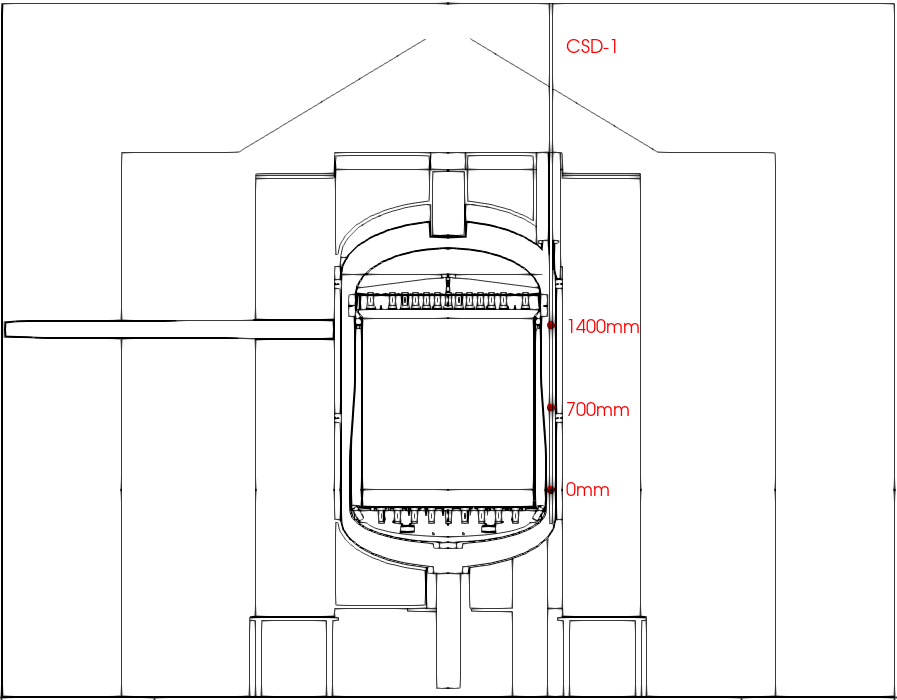
\includegraphics[width=\textwidth]{Figures/Geometry/csd1_geometry_black_and_white.png}
\caption{LZ geometry slice as implemented in GEANT4 from the water tank in. CSD-1 is shown along with the relevant Z-positions for calibration runs.}
\label{fig:CSD1_Geometry}
\end{figure}


\par
As the neutrons now originate outside of the TPC the \textbf{SS} had to be implemented.
The \textbf{SS} was defined as a cluster of activity close enough together that it cannot be distinguished if the deposits were turned into S1 and S2 signals.
It was defined as the energy-weighted variance in position being less than the detector spatial resolution.
This was determined from the result from LUX \cite{lux_position_reconstruction_ref}, scaled to LZ as per \cite{LZ_TechnicalDesignReview_ref} to give; ${\sigma}_{z}<0.2$ cm and ${\sigma}_{r}<3.0$ cm.
The \textbf{FID} is handled as before.
The result of the simulations is shown in \autoref{fig:simulated_amli_neutron_efficiency}.
\begin{figure}[]%
\centering
\begin{tikzpicture}
\centering
    \begin{groupplot}[%view={0}{90},
    group style = {group size = 1 by 3,vertical sep=1.5cm}]
    \nextgroupplot[
            %xlabel=Veto Window ($\mu$s),
            ylabel=Efficiency (\%),
            width=15cm, height=6cm,
            xmin=0, xmax=1000,
            ymin=85, ymax=100,
            minor y tick num=4,
            grid=major,
            legend style = { column sep = 10pt, legend columns = -1, legend to name = Simulated_AmLi_CommonLegend,}]
            \addplot+[green, mark=none]
                    table [x=Time,y=Efficiency]
                    {Data/Neutron_Efficiency/Simulation/edep_amli_neutron_eff_0mm_threshold_0.dat};
            \addplot[green, only marks, mark size=2pt,
                     error bar legend,
                     error bars/.cd,
                     x dir=both, x explicit, error bar style={color=black}]
                    table [x=Time,y=Efficiency, x error=EfficiencyError]
                    {Data/Neutron_Efficiency/Simulation/edep_amli_neutron_eff_0mm_threshold_0.dat};
                    
            \addplot+[blue, mark=none]
                    table [x=Time,y=Efficiency]
                    {Data/Neutron_Efficiency/Simulation/edep_amli_neutron_eff_0mm_threshold_100.dat};
            \addplot[blue, only marks, mark size=2pt,
                     error bar legend,
                     error bars/.cd,
                     x dir=both, x explicit, error bar style={color=black}]
                    table [x=Time,y=Efficiency, x error=EfficiencyError]
                    {Data/Neutron_Efficiency/Simulation/edep_amli_neutron_eff_0mm_threshold_100.dat};
                    
            \addplot+[red, mark=none]
                    table [x=Time,y=Efficiency]
                    {Data/Neutron_Efficiency/Simulation/edep_amli_neutron_eff_0mm_threshold_200.dat};
            \addplot[red, only marks, mark size=2pt,
                     error bar legend,
                     error bars/.cd,
                     x dir=both, x explicit, error bar style={color=black}]
                    table [x=Time,y=Efficiency, x error=EfficiencyError]
                    {Data/Neutron_Efficiency/Simulation/edep_amli_neutron_eff_0mm_threshold_200.dat};
            \node[draw, fill=white] at (axis cs: 800,87) {\large 0 mm};
            \legend{,0keV,,100keV,,200keV}
        
        \nextgroupplot[
            %xlabel=Veto Window ($\mu$s),
            ylabel=Efficiency (\%),
            width=15cm, height=6cm,
            xmin=0, xmax=1000,
            ymin=85, ymax=100,
            minor y tick num=4,
            grid=major,]
            \addplot+[green, mark=none]
                    table [x=Time,y=Efficiency]
                    {Data/Neutron_Efficiency/Simulation/edep_amli_neutron_eff_700mm_threshold_0.dat};
            \addplot[green, only marks, mark size=2pt,
                     error bar legend,
                     error bars/.cd,
                     x dir=both, x explicit, error bar style={color=black}]
                    table [x=Time,y=Efficiency, x error=EfficiencyError]
                    {Data/Neutron_Efficiency/Simulation/edep_amli_neutron_eff_700mm_threshold_0.dat};
                    
            \addplot+[blue, mark=none]
                    table [x=Time,y=Efficiency]
                    {Data/Neutron_Efficiency/Simulation/edep_amli_neutron_eff_700mm_threshold_100.dat};
            \addplot[blue, only marks, mark size=2pt,
                     error bar legend,
                     error bars/.cd,
                     x dir=both, x explicit, error bar style={color=black}]
                    table [x=Time,y=Efficiency, x error=EfficiencyError]
                    {Data/Neutron_Efficiency/Simulation/edep_amli_neutron_eff_700mm_threshold_100.dat};
                    
            \addplot+[red, mark=none]
                    table [x=Time,y=Efficiency]
                    {Data/Neutron_Efficiency/Simulation/edep_amli_neutron_eff_700mm_threshold_200.dat};
            \addplot[red, only marks, mark size=2pt,
                     error bar legend,
                     error bars/.cd,
                     x dir=both, x explicit, error bar style={color=black}]
                    table [x=Time,y=Efficiency, x error=EfficiencyError]
                    {Data/Neutron_Efficiency/Simulation/edep_amli_neutron_eff_700mm_threshold_200.dat};
            
             \node[draw, fill=white] at (axis cs: 800,87) {\large 700 mm};
        
        \nextgroupplot[
            xlabel=Veto Window ($\mu$s),
            ylabel=Efficiency (\%),
            width=15cm, height=6cm,
            xmin=0, xmax=1000,
            ymin=85, ymax=100,
            minor y tick num=4,
            grid=major,]
            \addplot+[green, mark=none]
                    table [x=Time,y=Efficiency]
                    {Data/Neutron_Efficiency/Simulation/edep_amli_neutron_eff_1400mm_threshold_0.dat};
            \addplot[green, only marks, mark size=2pt,
                     error bar legend,
                     error bars/.cd,
                     x dir=both, x explicit, error bar style={color=black}]
                    table [x=Time,y=Efficiency, x error=EfficiencyError]
                    {Data/Neutron_Efficiency/Simulation/edep_amli_neutron_eff_1400mm_threshold_0.dat};
                    
            \addplot+[blue, mark=none]
                    table [x=Time,y=Efficiency]
                    {Data/Neutron_Efficiency/Simulation/edep_amli_neutron_eff_1400mm_threshold_100.dat};
            \addplot[blue, only marks, mark size=2pt,
                     error bar legend,
                     error bars/.cd,
                     x dir=both, x explicit, error bar style={color=black}]
                    table [x=Time,y=Efficiency, x error=EfficiencyError]
                    {Data/Neutron_Efficiency/Simulation/edep_amli_neutron_eff_1400mm_threshold_100.dat};
                    
            \addplot+[red, mark=none]
                    table [x=Time,y=Efficiency]
                    {Data/Neutron_Efficiency/Simulation/edep_amli_neutron_eff_1400mm_threshold_200.dat};
            \addplot[red, only marks, mark size=2pt,
                     error bar legend,
                     error bars/.cd,
                     x dir=both, x explicit, error bar style={color=black}]
                    table [x=Time,y=Efficiency, x error=EfficiencyError]
                    {Data/Neutron_Efficiency/Simulation/edep_amli_neutron_eff_1400mm_threshold_200.dat};
            
             \node[draw, fill=white] at (axis cs: 800,87) {\large 1400 mm};
             
    \end{groupplot}
     \node at ($(group c1r1) + (-0.5cm, 3.0cm)$) {\ref{Simulated_AmLi_CommonLegend}};
\end{tikzpicture}
    \caption{Efficiency of the OD to veto neutrons from simulated AmLi neutron.}
    \label{fig:simulated_amli_neutron_efficiency}
\end{figure}




%\nextgroupplot[
%    xlabel=Veto Window ($\mu$s),
%    ylabel=Efficiency (\%),
%    width=15cm, height=6cm,
%    xmin=0, xmax=1000,
%    ymin=85, ymax=100,
%    minor y tick num=4,
%    grid=major,
%    legend style = { column sep = 10pt, legend columns = -1, legend to name = Simulated_AmLi_CommonLegend,}]
%    \addplot+[green, mark=none]
%            table [x=Time,y=Efficiency]
%            {Data/Neutron_Efficiency/Simulation/edep_amli_neutron_eff_amli_edeps_threshold_0kev_error_bars.dat};
%    \addplot[green, only marks, mark size=2pt,
%             error bar legend,
%             error bars/.cd,
%             x dir=both, x explicit, error bar style={color=black}]
%            table [x=Time,y=Efficiency, x error=EfficiencyError]
%            {Data/Neutron_Efficiency/Simulation/edep_amli_neutron_eff_amli_edeps_threshold_0kev_error_bars.dat};
%            
%    \addplot+[blue, mark=none]
%            table [x=Time,y=Efficiency]
%            {Data/Neutron_Efficiency/Simulation/edep_amli_neutron_eff_amli_edeps_threshold_100kev_error_bars.dat};
%    \addplot[blue, only marks, mark size=2pt,
%             error bar legend,
%             error bars/.cd,
%             x dir=both, x explicit, error bar style={color=black}]
%            table [x=Time,y=Efficiency, x error=EfficiencyError]
%            {Data/Neutron_Efficiency/Simulation/edep_amli_neutron_eff_amli_edeps_threshold_100kev_error_bars.dat};
%            
%    \addplot+[red, mark=none]
%            table [x=Time,y=Efficiency]
%            {Data/Neutron_Efficiency/Simulation/edep_amli_neutron_eff_amli_edeps_threshold_200kev_error_bars.dat};
%    \addplot[red, only marks, mark size=2pt,
%             error bar legend,
%             error bars/.cd,
%             x dir=both, x explicit, error bar style={color=black}]
%            table [x=Time,y=Efficiency, x error=EfficiencyError]
%            {Data/Neutron_Efficiency/Simulation/edep_amli_neutron_eff_amli_edeps_threshold_200kev_error_bars.dat};

%\par
%The efficiency for an AmLi source at 0 mm is the first time the 95\% veto efficiency requirement is not met, yet it is met for 1400 mm despite appearing to be in geometrically similar locations.
%The difference can be accounted for in the reduced volume of the BATs compared to TATs + YBe plug, with the area below the OCV being occupied by steel legs, water and foam.

\par
The veto efficiency varies depending upon the height of the source.
This can be understood by looking at the time it takes for the neutron to be captured.
For each of the 3 positions the neutron capture time is shown in \autoref{fig:simulated_amli_capture_time}.
The time it takes for a neutron to capture in a medium is modelled by an exponent in homogeneous media.
As the neutrons here travel through many different materials, the journey is significantly more complex.
Fortunately, this can still be approximated as just the sum of several exponents \cite{Dayabay_neutron_capture_fit_ref}.
Rather than a capture constant, $\tau$, representing the capture time in each volume, it is a constant representing the neutron path.
In the OD, the neutron capture time in GdLS distribution is given by:
\begin{equation}
    N(t) = \sum_{i} c_i \cdot e^{\frac{-t}{t_i}}
\label{eq:neutron_capture_time}
\end{equation}
The distributions in \autoref{fig:simulated_amli_capture_time} are best described by 3 terms the values.
The $\tau$ values for each location are summarised in \autoref{tab:simulated_neutron_capture_time}.
$\tau_1$ represented when the neutron spends almost all of its pre-capture time in the GdLS.
It is slightly above the GdLS capture time of $\backsim$28 $\mu$s \cite{ucsb_gdls_dicebox_simulations_ref} which is due to the neutron having to travel through some amount of non-GdLS first.
\par
Materials with a high H content, such as foam and acrylic, can effectively moderate and bound the neutron in that material.
It does, however, take a long time for the neutrons to capture in these mediums, which from simulations are 1450 $\mu$s and 240 $\mu$s, respectively.
The neutron can still escape and enter the GdLS to be captured.
$\tau_2$ and $\tau_3$ are from these processes, where the neutron is delayed entering the GdLS.
The effect on the capture time in the GdLS is shown on a per-volume basis in \autoref{fig:gdls_capture_time_vs_volume}.

\begin{table}[]
    \centering
    \begin{tabular}{c|c|c|c}
        Position  &  $\tau_1$      & $\tau_2$       & $\tau_3$        \\ \hline
        0 mm      & 30.54$\pm$0.29 & 63.42$\pm$2.70 & 139.3$\pm$3.1   \\ 
        700 mm    & 31.19$\pm$0.19 & 70.14$\pm$1.42 & 176.4$\pm$3.2   \\
        1400 mm   & 31.03$\pm$0.22 & 69.64$\pm$1.48 & 209.2$\pm$2.7         
    \end{tabular}
    \caption{Neutron capture time in GdLS from AmLi simulations where the source is in CSD-1 at three different locations.}
    \label{tab:simulated_neutron_capture_time}
\end{table}

\begin{figure}[]%
\centering
\begin{tikzpicture}
\centering
    \begin{axis}[
            xlabel=Time ($\mu$s),
            ylabel=Normalised Count,
            width=15cm,
            height=8cm,
            grid=major,
            xmin=0, xmax=1500,
            ymode=log, ymin=1e-7
            %legend style={at={(50.0,9.0)},anchor=north west},
            ]
            
            \addplot[blue, const plot]
                    table [x=time,y=count]
                    {Data/GdLS_Physics/neutron_capture_time/amli_capture_time_z0mm.dat};
            
            \addplot[red, const plot]
                    table [x=time,y=count]
                    {Data/GdLS_Physics/neutron_capture_time/amli_capture_time_z700mm.dat};
            
            \addplot[green, const plot]
                    table [x=time,y=count]
                    {Data/GdLS_Physics/neutron_capture_time/amli_capture_time_z1400mm.dat};
            
            % 0mm
            % \addplot[black,
            %      domain=15:1500,
            %      forget plot,
            %      ]
            % {1.216 * exp(-x/30.4) + 0.175 * exp(-x/61.95) + 0.02278 * exp(-x/137.1)}; 
            % 
            % \addplot[black,
            %      domain=15:1500,
            %      forget plot,
            %      ]
            % {1.282 * exp(-x/31.2) + 0.1314 * exp(-x/70.14) + 0.00667 * exp(-x/176.4)}; 
            % 
            % \addplot[red,
            %      domain=15:1500,
            %      forget plot,
            %      ]
            % {2305 * exp(-x/30.5) + 342 * exp(-x/125.2) + 0.9663}; 
            
            \legend{0mm, 700mm, 1400mm};
            
        
    \end{axis}
\end{tikzpicture}
\caption{Simulated neutron capture time in the GdLS for AmLi neutron events starting in CSD-1 at three heights.}
\label{fig:simulated_amli_capture_time}
\end{figure}

\begin{figure}[]
\centering
\begin{tikzpicture}
\begin{groupplot}[%
    group style={group size= 2 by 3, vertical sep=2.5cm,
    vertical sep=2.0cm},
    view={0}{90}
    %legend entries = {plot1,plot2}
    ]

    % Plot 2
    \nextgroupplot[width=0.45\textwidth,
                  ylabel=Volume time / Capture Time, ]
    \addplot3[
        point meta min=-6,
        point meta max=0,
		surf,
		shader=flat corner,
		colorbar right,
		colorbar style={ylabel={Portion in Volume}},
		mesh/cols=81,
		mesh/ordering=rowwise,
	   point meta = {z>1 ? nan : z}
		] file {Data/GdLS_Physics/capture_time_vs_volumes/volume_capture_times_ScintillatorCenter.dat};
	\node[draw, fill=white] at (axis cs: 1400,0.9) {\large GdLS};
		
	\nextgroupplot[colorbar, width=0.45\textwidth, colorbar style={ytick={-6,-5,...,0},}]
    \addplot3[
        point meta min=-6,
        point meta max=0,
		surf,
		shader=flat corner,
		mesh/cols=81,
		mesh/ordering=rowwise,
		point meta = {z>1 ? nan : z}
		] file {Data/GdLS_Physics/capture_time_vs_volumes/volume_capture_times_FoamDisplacer.dat};
	\node[draw, fill=white] at (axis cs: 1400,0.9) {\large OD Foam};
		
	\nextgroupplot[width=0.45\textwidth,
	               ylabel=Volume time / Capture Time,]
    \addplot3[
        point meta min=-4.5,
        point meta max=0,
        surf,
		shader=flat corner,
		colorbar right,
		colorbar style={ylabel={Portion in Volume}},
		mesh/cols=81,
		mesh/ordering=rowwise,
	   point meta = {z>1 ? nan : z}
		] file {Data/GdLS_Physics/capture_time_vs_volumes/volume_capture_times_WaterAndPMTs.dat};
    \node[draw, fill=white] at (axis cs: 1400,0.9) {\large OD Water};		
		
	\nextgroupplot[colorbar, width=0.45\textwidth, colorbar style={ytick={-6,-5,...,0},}]
    \addplot3[
		point meta min=-6,
        point meta max=0,
        surf,
		shader=flat corner,
		mesh/cols=81,
		mesh/ordering=rowwise,
		point meta = {z>1 ? nan : z}
		] file {Data/GdLS_Physics/capture_time_vs_volumes/volume_capture_times_ScintillatorTank.dat};
	\node[draw, fill=white] at (axis cs: 1400,0.9) {\large Acrylic Tanks};
		
	\nextgroupplot[width=0.45\textwidth,
	               ylabel=Volume time / Capture Time,
	               xlabel=Capture Time ($\mu$s),]
    \addplot3[
        point meta min=-6,
        point meta max=0,
        surf,
		shader=flat corner,
		colorbar right,
		colorbar style={ylabel={Portion in Volume}},
		mesh/cols=81,
		mesh/ordering=rowwise,
	   point meta = {z>1 ? nan : z}
		] file {Data/GdLS_Physics/capture_time_vs_volumes/volume_capture_times_LiquidXenonTarget.dat};
    \node[draw, fill=white] at (axis cs: 1400,0.9) {\large TPC Xenon};
		
	\nextgroupplot[colorbar, width=0.45\textwidth, colorbar style={ytick={-6,-5,...,0},},
	               xlabel=Capture Time ($\mu$s),]
    \addplot3[
        point meta min=-6,
        point meta max=0,
        surf,
		shader=flat corner,
		mesh/cols=81,
		mesh/ordering=rowwise,
		point meta = {z>1 ? nan : z}
		] file {Data/GdLS_Physics/capture_time_vs_volumes/volume_capture_times_LiquidSkinXenon.dat};
	\node[draw, fill=white] at (axis cs: 1400,0.9) {\large Skin Xenon};
	
\end{groupplot}
\end{tikzpicture}
\caption{Fraction of time spent in various detector regions against the capture time in the GdLS. Here OD Foam refers to all displacement foam between the OCV and acrylic tanks.}
\label{fig:gdls_capture_time_vs_volume}
\end{figure}

\par
In practice, any energy deposit will have to result in optical photons, which are subject to the light collection efficiency (shown in \autoref{fig:od_lce}) for a photon to reach a PMT and the efficiency of the PMT to generate a signal (shown in \autoref{fig:od_detection_properties}).
In order to determine the effect of this, full model simulations were performed for a single AmLi calibration position at the 700 mm level.
This position was chosen as the energy deposit efficiency was closest to that of a 1 MeV neutron.

\par
As these simulations resulted in a detector signal, the full suite of LZ analysis tools were used, where the simulated waveforms from PMTs are run through a pulse finding algorithm and interaction finder to identify single scatters.
The TPC contents of the event are reconstructed within the analysis package, providing both energy and position information of the event, making the application of the analysis cuts straightforward \cite{lz_simulations_ref}.
The OD veto energy threshold values were converted from energy to signal size using the values from a previous mock data challenge which are detailed in \cite{jonathannikoleyczik_thesis_ref}.
Additionally, a PMT multiplicity cut was included.
It was set such that 5 or more PMTs needed to contribute to the waveform in order for the pulse to be considered real.
This was implemented to account for PMT effects, such as after pulsing and dark counts \cite{jonathannikoleyczik_thesis_ref}.
However, no actual PMT effects were included in this simulation.
The result of this is shown in \autoref{fig:simulated_amli_full_propagation_efficiency} for AmLi at 700 mm. 

\par
The neutron efficiency in this case never reaches the performance requirement at any energy threshold, reducing to 91\% for a 200 keV threshold with a 500 $\mu$s window.
This indicates that the 95\% veto requirement will not be met by the LZ OD.
This is a slightly surprising result given the high efficiency measured earlier in this section.
However, this is the first time that optical propagation has been done to measure the efficiency, so is the first time that both the PMT quantum efficiency and light collection efficiency have really been considered.
In the next chapter analysis of an AmLi calibration campaign is performed to measure the true veto efficiency.

\begin{figure}[!htbp]%
\centering
\begin{tikzpicture}
\centering
    \begin{axis}[
            xlabel=Energy (MeV),
            ylabel=Probability,
            width=15cm,
            height=8cm,
            grid=major,
            xmin=0, xmax=1000,
            ymin=85, ymax=100,
            %legend style={at={(50.0,9.0)},anchor=north west},
            ]
            \addplot+[green, mark=none]
                    table [x=Time,y=Efficiency]
                    {Data/Neutron_Efficiency/Simulation/amli_neutron_eff_0kev_error_bars.dat};
            \addplot[green, only marks, mark size=2pt,
                     error bar legend,
                     error bars/.cd,
                     x dir=both, x explicit, error bar style={color=black}]
                    table [x=Time,y=Efficiency, x error=EfficiencyError]
                    {Data/Neutron_Efficiency/Simulation/amli_neutron_eff_0kev_error_bars.dat};
            \addplot+[blue, mark=none]
                    table [x=Time,y=Efficiency]
                    {Data/Neutron_Efficiency/Simulation/amli_neutron_eff_50kev_error_bars.dat};
            \addplot[blue, only marks, mark size=2pt,
                     error bar legend,
                     error bars/.cd,
                     x dir=both, x explicit, error bar style={color=black}]
                    table [x=Time,y=Efficiency, x error=EfficiencyError]
                    {Data/Neutron_Efficiency/Simulation/amli_neutron_eff_50kev_error_bars.dat};
            \addplot+[red, mark=none]
                    table [x=Time,y=Efficiency]
                    {Data/Neutron_Efficiency/Simulation/amli_neutron_eff_100kev_error_bars.dat};
            \addplot[red, only marks, mark size=2pt,
                     error bar legend,
                     error bars/.cd,
                     x dir=both, x explicit, error bar style={color=black}]
                    table [x=Time,y=Efficiency, x error=EfficiencyError]
                    {Data/Neutron_Efficiency/Simulation/amli_neutron_eff_100kev_error_bars.dat};
            \legend{,0keV,,100keV,,200keV}
            \end{axis}
\end{tikzpicture}
    \caption{Simulated AmLi neutron tagging efficiency for CSD-1 at 700mm.}
    \label{fig:simulated_amli_full_propagation_efficiency}
\end{figure}


\iffalse
The both the pure-LS and GdLS neutron capture times are well measured, with the most applicable for LZ from DayaBay, where the capture was modelled by \autoref{eq:neutron_capture_time} (Equation 15 in \cite{Dayabay_neutron_capture_fit_ref});
\begin{equation}
    N_{Gd}(t) = N_{0,Gd} \times [(1+\alpha)\frac{1}{\tau_{Gd}}e^{\frac{-1}{\tau_{Gd}}} - \alpha\frac{1}{\tau_{0}}e^{\frac{-t}{\tau_{0}}}] + C_{1} \\
\label{eq:neutron_capture_time}
\end{equation}
where the gadolinium capture can be constrained by two time constants $\tau_{Gd}$, which represents the capture of thermal neutrons and $\tau_{0}$ for neutrons captured before thermalisation\footnote{This is actually neutrons from inverse $\beta$-decay with energies $\mathcal{O}$(0.015)MeV being captured before scattering enough to thermalise.}. 
$\alpha$ is simply a there to balance to two terms.

\cite{snoplus_neutron_capture_time_on_water_ref}
\fi